\setlength{\parskip}{1em}
\setlength{\parindent}{0pt}
\chapter{L'applicazione OpenLDAT}
\label{chap:app}

Questo capitolo si concentra sull'applicazione OpenLDAT per PC, illustrandone i requisiti, le tecnologie utilizzate, e i dettagli del funzionamento, con un focus particolare agli algoritmi che analizzano i dati raccolti dal dispositivo.

I requisiti principali per l'applicazione OpenLDAT sono i seguenti:
\begin{itemize}
	\item Implementare dei test che utilizzano il dispositivo OpenLDAT per raccogliere dati e li analizzano per estrarre informazioni
	\item I test implementati devono essere il più possibile rappresentativi dell'utilizzo reale del sistema
	\item Funzionare su più sistemi operativi, almeno GNU/Linux, Windows e MacOS
	\item Essere facile da installare e utilizzare anche per un utente poco esperto
\end{itemize}

Prima di iniziare lo sviluppo sono state prese in considerazione più tecnologie per implementare l'applicazione: inizialmente sono stati fatti degli esperimenti con Electron, che oggi è molto popolare per sviluppare applicazioni desktop multipiattaforma, ma si sono presto presentate difficoltà dovute al fatto che l'engine Chromium al suo interno introduce esso stesso un notevole ritardo di input, per cui i test non sarebbero stati rappresentativi; la scelta finale è quindi ricaduta su Java SE con OpenGL, scelta che consente molta più libertà di implementazione, e di realizzare quindi test più rappresentativi di un utilizzo reale.

L'applicazione è strutturata in quattro parti principali più alcune classi di utilità:
\begin{itemize}
	\item \textbf{Comunicazione con il dispositivo} (package \texttt{com.dosse.openldat.device}): è sostanzialmente un driver per il dispositivo OpenLDAT che ha il compito di rilevare il dispositivo e consentire al resto dell'applicazione di utilizzarlo in modo semplice, senza preoccuparsi dei dettagli di comunicazione
	\item \textbf{Elaborazione di base} (package \texttt{com.dosse.openldat.processing}): fornisce un insieme di strumenti per memorizzare i dati in arrivo dal dispositivo e dei filtri che possono essere applicati su di essi (ad esempio, FFT)
	\item \textbf{I test} (package \texttt{com.dosse.openldat.tests}): questa è la parte principale dell'applicazione e implementa tutti i test che sono stati sviluppati per OpenLDAT, oltre a due backend grafiche per disegnare sullo schermo con e senza OpenGL
	\item \textbf{La GUI} (package \texttt{com.dosse.openldat.ui}): implementa l'interfaccia grafica per l'applicazione che permette di configurare ed eseguire i test e visualizzarne in modo grafico i risultati
\end{itemize}

Oltre a Java SE, per lo sviluppo dell'applicazione sono state utilizzate anche le seguenti librerie:
\begin{itemize}
	\item \textbf{jSerialComm} \footnote{\href{https://github.com/Fazecast/jSerialComm}{https://github.com/Fazecast/jSerialComm}}: una libreria che consente ad applicazioni Java di interfacciarsi con dispositivi seriali
	\item \textbf{LWJGL} \footnote{\href{https://www.lwjgl.org/}{https://www.lwjgl.org/}}: una libreria per lo sviluppo di applicazioni OpenGL in Java, utilizzata anche da giochi commerciali come Minecraft
	\item \textbf{JTransforms} \footnote{\href{https://github.com/wendykierp/JTransforms}{https://github.com/wendykierp/JTransforms}}: utilizzata per realizzare il filtro FFT
\end{itemize}

Tutti i file relativi all'applicazione e al packaging per le varie piattaforme sono presenti nella cartella \texttt{App} all'interno del repository. Il progetto \texttt{OpenLDAT} al suo interno può essere caricato in NetBeans IDE.

Nelle sezioni successive verranno discussi approfonditamente tutti gli aspetti dell'applicazione.

\section{Comunicazione col dispositivo}
Questa sezione si concentra sul package \texttt{com.dosse.openldat.device}, che implementa tutta la parte di comunicazione con il dispositivo OpenLDAT.

\subsection{DeviceFinder}
La comunicazione col dispositivo avviene tramite l'interfaccia seriale USB esposta dal dispositivo, ma prima di poter comunicare con esso, bisogna trovarlo. Poiché al PC potrebbero essere connessi più dispositivi seriali, l'applicazione distingue i dispositivi OpenLDAT dagli altri grazie all'ID hardware impostato dal firmware come spiegato nel capitolo precedente.
Il processo di discovery dei dispositivi è svolto dalla classe \texttt{DeviceFinder}, la quale contiene dei metodi statici per trovare i dispositivi.

\paragraph{Metodi statici:}\begin{itemize}
	\item \texttt{public static SerialPort[] findDevices()}: trova tutti i dispositivi OpenLDAT attualmente connessi e li ritorna come un array di \texttt{SerialPort} (una classe della libreria jSerialComm). Non viene fatto alcun controllo sullo stato del dispositivo stesso, nè del fatto che sia supportato o meno
	\item \texttt{public static Device getDevice()}: un metodo più comodo per ottenere il primo device OpenLDAT connesso al PC supportato dall'applicazione, o \texttt{null} se non ce ne sono. Questo metodo è utile solo per comodità in fase di testing, l'applicazione non lo utilizza. Il metodo ritorna un'istanza di \texttt{Device}, che è la classe che implementa effettivamente la comunicazione con il dispositivo
\end{itemize}

\subsection{Device}
Una volta scelto il dispositivo OpenLDAT da utilizzare, si può istanziare la classe \texttt{Device} passandole la porta seriale scelta. Il costruttore di questa classe esegue tutti i controlli necessari per identificare il dispositivo, verificare che sia supportato, e ottiene l'elenco delle capability. In seguito, la classe mette a disposizione dei metodi per utilizzare il dispositivo. La classe utilizza un buffer in ricezione di 128kB per evitare di bloccare il dispositivo mentre qualcosa viene processato.

\paragraph{Costruttori:}\begin{itemize}
	\item \texttt{public Device(SerialPort com)}: crea l'istanza di \texttt{Device} utilizzando la porta seriale specificata. Durante l'inizializzazione, viene verificato il modello del dispositivo e viene richiesto l'elenco delle capability per inizializzare tutte le variabili interne alla classe. Se il dispositivo non è riconosciuto, non è compatibile, richiede una versione più recente del driver, o l'elenco delle capability non è valido, l'inizializzazione fallisce.\\
	Il costruttore può lanciare un'eccezione \texttt{DeviceError} se l'inizializzazione fallisce o una \texttt{IOException} se ci sono problemi di comunicazione durante l'inizializzazione
\end{itemize}

\paragraph{Metodi pubblici:}\begin{itemize}
	\item \texttt{public boolean isOpen()}: ritorna \texttt{true} se la connessione al dispositivo è attualmente aperta
	\item \texttt{public void close()}: chiude la connessione verso il dispositivo in modo sicuro, terminando qualsiasi attività in corso
	\item \texttt{public boolean hasLightSensor()}: ritorna \texttt{true} se il dispositivo è dotato di un sensore di luminosità
	\item \texttt{public boolean isPrototype()}: ritorna \texttt{true} se il dispositivo si dichiara come prototipo. Nella GUI, i prototipi hanno a disposizione un menu di test dedicato
	\item \texttt{public boolean hasOscilloscopeDebug()}: ritorna \texttt{true} se il dispositivo genera pulsazioni sul pin 10 durante l'attività
	\item \texttt{public String getFirmwareVersion()}: ritorna la versione del firmware come una stringa. Per convenzione, le versioni del firmware contengono la data in formato YYYYMMDD seguita opzionalmente da altri caratteri, ad esempio \texttt{20210225-production}
	\item \texttt{public String getModel()}: ritorna il modello completo del dispositivo come dichiarato dal firmware, non dall'ID hardware
	\item \texttt{public int getModelCode()}: ritorna il modello del dispositivo come numero. Attualmente, il dispositivo OpenLDAT Model 1 è l'unico supportato ed ha il codice 1
	\item \texttt{public String getPortName()}: ritorna il nome della porta seriale del dispositivo
	\item \texttt{public int getMinDriverVersion()}: ritorna il codice di versione minimo del driver richiesto dal dispositivo come dichiarato dal firmware. La versione attuale del driver ha codice di versione 1
	\item \texttt{public String getSerialNumber()}: ritorna il numero di serie del dispositivo come stringa, o la stringa \texttt{DIY} se non ce l'ha
	\item \texttt{public boolean isBusy()}: ritorna \texttt{true} se il dispositivo sta eseguendo qualche attività ed è occupato
	\item \texttt{public void endCurrentActivity()}: termina l'attività corrente e attende che il dispositivo torni in stato idle per accettare nuovi comandi. Questo metodo è bloccante fino a quando il dispositivo non è in stato idle. L'esecuzione richiede circa 100ms. Questo metodo va utilizzato solo per interrompere un'attività (ad esempio alla fine di un test), se si desidera passare da un'attività a un'altra, quella precedente viene interrotta automaticamente dalla nuova
	\item \texttt{public double lightSensorMonitorMode(boolean noBuffer, byte sensitivity, boolean fastADC, LightSensorMonitorCallback callback)}: avvia il campionamento del sensore di luminosità sul dispositivo, senza pulsante.\begin{itemize}
		\item \texttt{boolean noBuffer}: se impostato a \texttt{true}, utilizza la modalità senza buffering (più lenta ma campionamento più regolare), altrimenti utilizza la modalità con buffering
		\item \texttt{byte sensitivity}: imposta il livello di gain del sensore tra 0 (più basso) e 3 (più alto)
		\item \texttt{boolean fastADC}: se impostato a \texttt{true}, campiona il segnale molto più velocemente
		\item \texttt{LightSensorMonitorCallback callback}: il callback da chiamare quando sono disponibili nuovi dati dal dispositivo. Questa classe verrà approfondita successivamente
	\end{itemize}
	Una volta avviato il campionamento il metodo non è bloccante, e ritorna il sample rate del segnale che sta acquisendo.\\
	Se il dispositivo non ha un sensore di luminosità viene lanciata un'eccezione \texttt{MissingSensorException}, se si verificano errori di comunicazione, viene lanciata una \texttt{IOException}.\\
	Se il metodo viene chiamato mentre è già in corso un'altra attività, questa viene terminata automaticamente e quella nuova viene eseguita
	\item \texttt{public double getLightSensorMonitorModeSampleRate(boolean noBuffer, boolean fastADC)}: ritorna la frequenza di campionamento che offrirebbe il dispositivo nel campionare il sensore di luminosità senza il pulsante, con le impostazioni richieste.\begin{itemize}
		\item \texttt{boolean noBuffer}: se impostato a \texttt{true}, utilizza la modalità senza buffering (più lenta ma campionamento più regolare), altrimenti utilizza la modalità con buffering
		\item \texttt{boolean fastADC}: se impostato a \texttt{true}, campiona il segnale molto più velocemente
	\end{itemize}
	Vedi anche: tabella \ref{tab:openldat_samplerates} (con \texttt{MONITOR=1}).\\
	Viene lanciata un'eccezione \texttt{MissingSensorException} se il dispositivo non ha un sensore di luminosità
	\item \texttt{public double lightSensorButtonMode(boolean noBuffer, byte sensitivity, boolean fastADC, boolean noClick, boolean autoFire, LightSensorButtonCallback callback)}: avvia il campionamento del sensore di luminosità sul dispositivo, con il pulsante.\begin{itemize}
		\item \texttt{boolean noBuffer}: se impostato a \texttt{true}, utilizza la modalità senza buffering (più lenta ma campionamento più regolare), altrimenti utilizza la modalità con buffering
		\item \texttt{byte sensitivity}: imposta il livello di gain del sensore tra 0 (più basso) e 3 (più alto)
		\item \texttt{boolean fastADC}: se impostato a \texttt{true}, campiona il segnale molto più velocemente
		\item \texttt{boolean noClick}: se impostato a \texttt{true}, i click vengono registrati ma non viene simulato un click del mouse
		\item \texttt{boolean autoFire}: se impostato a \texttt{true}, i click vengono generati automaticamente, altrimenti vengono ricevuti tramite il pulsante esterno
		\item \texttt{LightSensorButtonCallback callback}: il callback da chiamare quando sono disponibili nuovi dati dal dispositivo. Questa classe verrà approfondita successivamente
	\end{itemize}
	Una volta avviato il campionamento il metodo non è bloccante, e ritorna il sample rate del segnale che sta acquisendo.\\
	Se il dispositivo non ha un sensore di luminosità viene lanciata un'eccezione \texttt{MissingSensorException}, se si verificano errori di comunicazione, viene lanciata una \texttt{IOException}.\\
	Se il metodo viene chiamato mentre è già in corso un'altra attività, questa viene terminata automaticamente e quella nuova viene eseguita
	\item \texttt{public double getLightSensorButtonModeSampleRate(boolean noBuffer, boolean fastADC)}: ritorna la frequenza di campionamento che offrirebbe il dispositivo nel campionare il sensore di luminosità senza il pulsante, con le impostazioni richieste.\begin{itemize}
		\item \texttt{boolean noBuffer}: se impostato a \texttt{true}, utilizza la modalità senza buffering (più lenta ma campionamento più regolare), altrimenti utilizza la modalità con buffering
		\item \texttt{boolean fastADC}: se impostato a \texttt{true}, campiona il segnale molto più velocemente
	\end{itemize}
	Vedi anche: tabella \ref{tab:openldat_samplerates} (con \texttt{MONITOR=0}).\\
	Viene lanciata un'eccezione \texttt{MissingSensorException} se il dispositivo non ha un sensore di luminosità
\end{itemize}

\subsection{Callback e errori}
I package \texttt{com.dosse.openldat.device.callback} e \texttt{com.dosse.openldat.device.errors} contengono le classi che implementano i callback e gli errori menzionate precedentemente.

\subsubsection{DeviceError}
Questa classe estende \texttt{Exception} ed è usata per definire tutti gli errori che possono verificarsi all'interno di \texttt{Device}.

\paragraph{Costruttori:}\begin{itemize}
	\item \texttt{public DeviceError(int type)}: crea l'eccezione utilizzando uno dei tipi predefiniti nella classe stessa (\texttt{FAILED\_TO\_CONNECT}, \texttt{UNSUPPORTED\_MODEL}, \texttt{NOT\_OPENLDAT\_DEVICE}, \texttt{DEVICE\_ID\_FAILED}, \texttt{FIRMWARE\_BUILT\_WITH\_SERIALPLOT}, \texttt{FIRMWARE\_NEEDS\_NEWER\_DRIVER}, \texttt{FIRMWARE\_UNKNOWN}, \texttt{FIRMWARE\_LIGHTSENSOR\_MISSING\_BUFSIZES})
	\item \texttt{public DeviceError(String message)}: crea l'eccezione utilizzando un messaggio personalizzato
\end{itemize}

\paragraph{Metodi pubblici:}\begin{itemize}
	\item \texttt{public int getType()}: ritorna il tipo di eccezione specificata nel costruttore, oppure \texttt{CUSTOM\_ERROR} se è stata inizializzata con un messaggio personalizzato (ottenibile con \texttt{getMessage()})
\end{itemize}

\subsubsection{MissingSensorException}
Questa classe estende \texttt{Exception} ed è usata per gli errori in cui si cerca di utilizzare un sensore non presente sul dispositivo. Funziona in modo analogo a \texttt{DeviceError}.

\paragraph{Costruttori:}\begin{itemize}
	\item \texttt{public MissingSensorException(int type)}: crea l'eccezione utilizzando uno dei tipi predefiniti nella classe stessa (attualmente solo \texttt{LIGHT\_SENSOR})
	\item \texttt{public MissingSensorException(String message)}: crea l'eccezione utilizzando un messaggio personalizzato
\end{itemize}

\paragraph{Metodi pubblici:}\begin{itemize}
	\item \texttt{public int getType()}: ritorna il tipo di eccezione specificata nel costruttore, oppure \texttt{CUSTOM\_ERROR} se è stata inizializzata con un messaggio personalizzato (ottenibile con \texttt{getMessage()})
\end{itemize}

\subsubsection{LightSensorMonitorCallback}
Questa classe implementa i callback per il metodo \texttt{lightSensorMonitorMode} della classe \texttt{Device}. Non è obbligatorio fare l'override di tutti i metodi per utilizzarla.

\paragraph{Metodi pubblici:}\begin{itemize}
	\item \texttt{public void onDataBufferReceived(int[] data){}}: questo callback viene chiamato quando viene ricevuto un nuovo buffer di dati (ossia \texttt{noBuffer} è impostato a \texttt{false}). L'array \texttt{data} contiene i sample ricevuti dal dispositivo sotto forma di interi tra 0 e 1023. La lunghezza dell'array è sempre costante (32 sample).\\
	Attenzione: questo callback deve terminare il prima possibile per evitare di rallentare la lettura dal dispositivo
	\item \texttt{public void onDataSampleReceived(int data){}}: questo callback viene chiamato quando viene ricevuto un nuovo sample dal dispositivo (ossia \texttt{noBuffer} è impostato a \texttt{true}). Il sample è rappresentato con un intero tra 0 e 1023.\\
	Attenzione: questo callback deve terminare il prima possibile per evitare di rallentare la lettura dal dispositivo
	\item \texttt{public void onError(Exception e)}: questo callback viene chiamato se si verifica un errore, per esempio se il dispositivo viene disconnesso mentre si sta campionando. Se non si fa l'override di questo metodo, il suo comportamento di default è stampare l'eccezione e lo stacktrace
\end{itemize}

La scelta di tenere metodi separati per la gestione di un intero buffer e per la gestione dei singoli sample è stata fatta perché spesso è possibile applicare qualche tipo di ottimizzazione per ridurre il carico sulla CPU se si lavora su interi buffer anziché singoli sample.

\subsubsection{LightSensorButtonCallback}
Questa classe implementa i callback per il metodo \texttt{lightSensorButtonMode} della classe Device. Il suo funzionamento è analogo a quello di \texttt{LightSensorMonitorCallback}, ma oltre anziché ricevere solo la luce, si riceve anche lo stato del pulsante. Non è obbligatorio fare l'override di tutti i metodi per utilizzarla.

\paragraph{Metodi pubblici:}\begin{itemize}
	\item \texttt{public void onDataBufferReceived(int[] light, int[] click){}}: questo callback viene chiamato quando viene ricevuto un nuovo buffer di dati (ossia \texttt{noBuffer} è impostato a \texttt{false}). L'array \texttt{light} contiene i sample del sensore di luminosità sotto forma di interi tra 0 e 1023, mentre l'array \texttt{click} contiene i sample del pulsante sotto forma di interi tra 0 e 1. I due array hanno la stessa lunghezza. La lunghezza dei due array è sempre costante (21 sample).\\
	Attenzione: questo callback deve terminare il prima possibile per evitare di rallentare la lettura dal dispositivo
	\item \texttt{public void onDataSampleReceived(int light, int click){}}: questo callback viene chiamato quando viene ricevuto un nuovo sample dal dispositivo (ossia \texttt{noBuffer} è impostato a \texttt{true}). L'intero \texttt{light} contiene il valore di luminosità come intero tra 0 e 1023, mentre l'intero \texttt{click} contiene lo stato del pulsante come intero tra 0 e 1.\\
	Attenzione: questo callback deve terminare il prima possibile per evitare di rallentare la lettura dal dispositivo
	\item \texttt{public void onError(Exception e)}: questo callback viene chiamato se si verifica un errore, per esempio se il dispositivo viene disconnesso mentre si sta campionando. Se non si fa l'override di questo metodo, il suo comportamento di default è stampare l'eccezione e lo stacktrace
\end{itemize}

\subsection{Esempio di utilizzo}
Nel seguente listato viene mostrato come è possibile utilizzare le classi appena descritte per collegarsi al dispositivo e stampare i valori del sensore di luminosità e del pulsante sul terminale.
\lstinputlisting[language=Java]{Applicazione_files/DeviceExample.java}

\section{Elaborazione di base}
I dati catturati dal sensore, dopo che sono stati ricevuti, devono essere memorizzati per poter estrarre informazioni utili. Per fare questo, il package \texttt{com.dosse.openldat.processing} fornisce dei buffer e alcuni filtri per rendere più facile l'analisi che in seguito sarà svolta dal codice dei test.

\subsection{Buffer}
L'obiettivo dei buffer in questa applicazione è quello di memorizzare gli ultimi $N$ sample ricevuti, così da poterli analizzare in seguito, senza limiti di tempo.\\
Nel package \texttt{com.dosse.openldat.processing.buffers} vengono forniti due tipi di buffer e l'interfaccia generica per i buffer, che ora saranno discussi in dettaglio.

Nota: poiché tutti i dati ricevuti dal dispositivo sono numeri interi, i buffer sono pensati per memorizzare solo quelli, non fanno uso di generics.

\subsubsection{IBuffer}
L'interfaccia \texttt{IBuffer} definisce i metodi che tutti i buffer devono implementare.

\paragraph{Metodi da implementare:}\begin{itemize}
	\item \texttt{public void add(int val)}: aggiunge un singolo intero al buffer
	\item \texttt{public void add(int[] data)}: aggiunge un array di interi al buffer
	\item \texttt{public int[] getData()}: ritorna il contenuto attuale del buffer in maniera sicura (rispettando l'incapsulamento e in modo thread-safe)
	\item \texttt{public int[] getDataUnsafe()}: ritorna il contenuto attuale del buffer in maniera insicura (non rispetta l'incapsulamento e non è thread safe)
	\item \texttt{public int getSize()}: ritorna la dimensione del buffer, ossia quanti interi può contenere il buffer prima di sovrascrivere dei dati
	\item \texttt{public boolean isFilled()}: ritorna \texttt{true} se il buffer è pieno, ossia se sono già stati aggiunti abbastanza dati per evitare che ci siano celle vuote chiamando \texttt{getData}
\end{itemize}

\subsubsection{CircularBuffer}
Questa classe implementa una variante di un buffer circolare che permette di memorizzare gli ultimi $N$ sample aggiunti al buffer, con operazioni di aggiunta e lettura del buffer molto veloci.\\
Nonostante il nome, non è un buffer circolare in senso stretto, poiché il puntatore di scrittura e di lettura coincidono, ma questo è ciò di cui abbiamo bisogno per realizzare l'applicazione e velocizza notevolmente il codice.\\
Tutte le operazioni di questa classe utilizzano i metodi di copia di memoria del sistema anziché dei cicli, migliorando notevolmente le prestazioni.

La classe è thread-safe.

\paragraph{Costruttori:}\begin{itemize}
	\item \texttt{public CircularBuffer(int size)}: inizializza un buffer circolare di dimensione \texttt{size}
\end{itemize}

\paragraph{Metodi pubblici:}\begin{itemize}
	\item \texttt{public void add(int val)}: aggiunge un singolo intero al buffer. Se è pieno, viene sovrascritto il valore più vecchio
	\item \texttt{public void add(int[] data)}: aggiunge un array di interi al buffer. Se è pieno, vengono sovrascritti i valori più vecchi
	\item \texttt{public int[] getData()}: ritorna il contenuto attuale del buffer in maniera sicura (rispettando l'incapsulamento e in modo thread-safe)
	\item \texttt{public int[] getDataUnsafe()}: non supportato su un buffer circolare, esegue semplicemente \texttt{getData}
	\item \texttt{public int[] getInternalBuffer()}: ritorna l'array usato internamente per memorizzare i dati. I dati potrebbero non essere in ordine
	\item \texttt{public int getSize()}: ritorna la dimensione del buffer, ossia quanti interi può contenere il buffer prima di sovrascrivere dei dati
	\item \texttt{public boolean isFilled()}: ritorna \texttt{true} se il buffer è pieno, ossia se sono già stati aggiunti abbastanza dati per evitare che ci siano celle vuote chiamando \texttt{getData}
\end{itemize}

\subsubsection{ArrayBuffer}
Questa è implementa un buffer costante (non è possibile aggiungere nulla). Si tratta di una classe di utilità, utilizzata quando serve avere un array sotto forma di buffer.

La classe è thread-safe.

\paragraph{Costruttori:}\begin{itemize}
	\item \texttt{public ArrayBuffer(int[] data)}: inizializza il buffer con l'array di dati fornito. Nota: i dati non vengono copiati, ma solo il riferimento, per cui è possibile alterare il contenuto di questo buffer esternamente. Questo è voluto ed è utilizzato nella GUI
\end{itemize}

\paragraph{Metodi pubblici:}\begin{itemize}
	\item \texttt{public void add(int val)}: non supportato, lancia una \texttt{UnsupportedOperationException}
	\item \texttt{public void add(int[] data)}: non supportato, lancia una \texttt{UnsupportedOperationException}
	\item \texttt{public int[] getData()}: ritorna una copia dell'array \texttt{data} con cui è stato inizializzato il buffer
	\item \texttt{public int[] getDataUnsafe()}: ritorna l'array \texttt{data} con cui è stato inizializzato il buffer (riferimento)
	\item \texttt{public int getSize()}: ritorna la dimensione del buffer, ossia la dimensione dell'array \texttt{data} con cui è stato inizializzato
	\item \texttt{public boolean isFilled()}: ritorna sempre \texttt{true}
\end{itemize}

\subsection{Filtri}
Il package \texttt{com.dosse.openldat.processing.filters} contiene alcuni filtri che sono usati per semplificare l'analisi dei dati raccolti. A tutti gli effetti, un filtro non è altro che un tipo speciale di buffer, che però esegue un qualche tipo di elaborazione sui dati che gli vengono inseriti.

\subsubsection{FFTFilter}
Questa classe implementa un filtro che permette di inserire dati nel dominio del tempo (sample) e ottenere una rappresentazione degli stessi dati nel dominio di frequenza utilizzando una FFT (Fast Fourier Transform). La trasformazione viene eseguita dalla libreria jTransforms, ma prima viene applicata ai dati una funzione di windowing di Blackman-Harris, per generare dati più puliti. Per velocizzare l'esecuzione, l'FFT non viene eseguita ad ogni sample aggiunto, ma solo nel momento in cui vengono richiesti i dati.

\paragraph{Costruttori:}\begin{itemize}
	\item \texttt{public FFTFilter(int size)}: inizializza il filtro su un buffer circolare di dimensione \texttt{size}, che deve essere una potenza di 2 (requisito dell'FFT)
\end{itemize}

\paragraph{Metodi pubblici:} \begin{itemize}
	\item \texttt{public void add(int val)}: aggiunge un singolo intero al buffer. Se è pieno, viene sovrascritto il valore più vecchio
	\item \texttt{public void add(int[] data)}: aggiunge un array di interi al buffer. Se è pieno, vengono sovrascritti i valori più vecchi
	\item \texttt{public int[] getData()}: ritorna il contenuto attuale del buffer, ma nel dominio della frequenza. Ogni valore nell'array ritornato è un bin dell'FFT e il suo valore indica la potenza del segnale in quel bin. Per conoscere la frequenza a cui corrisponde l'i-esimo bin, è sufficiente usare la seguente formula: $\frac{i}{size}*(\frac{sampleRate}{2})$
	\item \texttt{public int[] getDataUnsafe()}: non supportato su un buffer circolare, esegue semplicemente \texttt{getData}
	\item \texttt{public int[] getOriginalData()}: ritorna i dati inseriti nel buffer, nel dominio temporale
	\item \texttt{public int[] getInternalBuffer()}: ritorna l'array usato internamente per memorizzare i dati nel dominio temporale. I dati potrebbero non essere in ordine
	\item \texttt{public int getSize()}: ritorna la dimensione del buffer, ossia quanti interi può contenere il buffer prima di sovrascrivere dei dati
	\item \texttt{public boolean isFilled()}: ritorna \texttt{true} se il buffer è pieno, ossia se sono già stati aggiunti abbastanza dati per evitare che ci siano celle nel buffer
\end{itemize}

\subsubsection{RunningAverageSmoothingFilter}
Questa classe implementa un filtro che ``smussa'' i dati utilizzando una sorta di media mobile.

Il filtro funziona in questo modo: internamente viene mantenuto il valore di output corrente che chiamiamo $currentValue$, inizializzato a 0; ogni volta che viene aggiunto un nuovo sample $new$, si aggiorna in questo modo: $currentValue=smoothing*currentValue+(1-smoothing)*new$, dove $smoothing$ è un valore tra 0 e 1 e indica la resistenza che il filtro oppone a cambiare il valore (0 è istantaneo, 1 non cambia mai). Valori tipici per $smoothing$ sono molto vicini a 1.

La classe è thread-safe.

\paragraph{Costruttori:} \begin{itemize}
	\item \texttt{public RunningAverageSmoothingFilter(int size, double smoothing)}: inizializza il filtro su un buffer circolare di dimensione \texttt{size} e con il valore di \texttt{smoothing}
\end{itemize}

\paragraph{Metodi pubblici:} \begin{itemize}
	\item \texttt{public void add(int val)}: aggiunge un singolo intero al buffer. Se è pieno, viene sovrascritto il valore più vecchio. Quando viene aggiunto il primo sample, il valore di $currentValue$ viene inizializzato con quel valore
	\item \texttt{public void add(int[] data)}: aggiunge un array di interi al buffer. Se è pieno, vengono sovrascritti i valori più vecchi. Quando viene aggiunto il primo sample, il valore di $currentValue$ viene inizializzato con quel valore
	\item \texttt{public int[] getData()}: ritorna il contenuto attuale del buffer in maniera sicura (rispettando l'incapsulamento e in modo thread-safe)
	\item \texttt{public int[] getDataUnsafe()}: non supportato su un buffer circolare, esegue semplicemente \texttt{getData}
	\item \texttt{public int[] getInternalBuffer()}: ritorna l'array usato internamente per memorizzare i dati. I dati potrebbero non essere in ordine
	\item \texttt{public int getSize()}: ritorna la dimensione del buffer, ossia quanti interi può contenere il buffer prima di sovrascrivere dei dati
	\item \texttt{public boolean isFilled()}: ritorna \texttt{true} se il buffer è pieno, ossia se sono già stati aggiunti abbastanza dati per evitare che ci siano celle vuote chiamando \texttt{getData}
\end{itemize}

\subsubsection{PeakHoldFilter}
Questa classe implementa un filtro che mantiene i picchi del segnale dato in ingresso. Ogni sample in output generato dal filtro contiene il valore massimo di una finestra di sample inseriti precedentemente. Questa classe è particolarmente utile per elaborare segnali misurati su display con retroilluminazione PWM.

La classe è thread-safe.

\paragraph{Costruttori:}\begin{itemize}
	\item \texttt{public PeakHoldFilter(int size, int peakWindowSize)}: inizializza il filtro con una dimensione del buffer di \texttt{size} e una dimensione della finestra in cui ricercare il massimo di \texttt{peakWindowSize}
\end{itemize}

\paragraph{Metodi pubblici:}\begin{itemize}
	\item \texttt{public void add(int val)}: aggiunge un singolo intero al buffer. Se è pieno, viene sovrascritto il valore più vecchio
	\item \texttt{public void add(int[] data)}: aggiunge un array di interi al buffer. Se è pieno, vengono sovrascritti i valori più vecchi
	\item \texttt{public int[] getData()}: ritorna il contenuto attuale del buffer in maniera sicura (rispettando l'incapsulamento e in modo thread-safe)
	\item \texttt{public int[] getDataUnsafe()}: non supportato su un buffer circolare, esegue semplicemente \texttt{getData}
	\item \texttt{public int[] getInternalBuffer()}: ritorna l'array usato internamente per memorizzare i dati. I dati potrebbero non essere in ordine
	\item \texttt{public int getSize()}: ritorna la dimensione del buffer, ossia quanti interi può contenere il buffer prima di sovrascrivere dei dati
	\item \texttt{public boolean isFilled()}: ritorna \texttt{true} se il buffer è pieno, ossia se sono già stati aggiunti abbastanza dati per evitare che ci siano celle vuote chiamando \texttt{getData}
\end{itemize}

\paragraph{Metodi statici:}\begin{itemize}
	\item \texttt{public static int findBestWindowSize(int[] noisyData, int min, int max, int stepSize, int noiseThreshold)}: determina il valore minimo di \texttt{peakWindowSize} da utilizzare per far si che applicando il filtro sull'array \texttt{noisyData}, la differenza tra il valore minimo e massimo dopo il filtraggio sia inferiore a \texttt{noiseThreshold}. \texttt{min} e \texttt{max} permettono di restringere l'intervallo di ricerca del valore di \texttt{peakWindowSize} in quel range, a passi di \texttt{stepSize}. Ritorna -1 se i dati in input non sono validi
\end{itemize}

\subsection{Esempio di utilizzo}
Il seguente listato mostra un esempio di come è possibile acquisire un segnale dal dispositivo e filtrarlo. I grafici nelle figure \ref{fig:filters_example_original}, \ref{fig:filters_example_smooth} e \ref{fig:filters_example_peakHold} mostrano l'output dei filtri. Il segnale catturato è un LED con una PWM di circa 120Hz con piccoli movimenti del sensore per mostrare meglio il comportamento dei filtri.
\lstinputlisting[language=Java]{Applicazione_files/FiltersExample.java}
\begin{figure}[H]
	\centering
	\begin{tikzpicture}
		\begin{axis}[name=Segnale, xmin=0,xmax=8192,ymin=0,ymax=1023,width=.8\textwidth,xlabel=Sample,ylabel=Valore]
			\addplot[black] file{Applicazione_files/filters_example_original.txt};
		\end{axis}
	\end{tikzpicture}
	\begin{tikzpicture}
		\begin{axis}[name=Spettro, xmin=0,xmax=4000,ymin=0,ymax=150000,width=.8\textwidth,xlabel=Frequenza (Hz),ylabel=Potenza]
			\addplot[black] file{Applicazione_files/filters_example_fft.txt};
		\end{axis}
	\end{tikzpicture}
	\caption{Segnale originale e relativo spettro in frequenza. I picchi sono causati dalla frequenza della PWM}
	\label{fig:filters_example_original}
\end{figure}
\begin{figure}[H]
	\centering
	\begin{tikzpicture}
		\begin{axis}[name=Segnale, xmin=0,xmax=8192,ymin=0,ymax=1023,width=.8\textwidth,xlabel=Sample,ylabel=Valore]
			\addplot[gray] file{Applicazione_files/filters_example_original.txt};
			\addplot[red] file{Applicazione_files/filters_example_smooth.txt};
		\end{axis}
	\end{tikzpicture}
	\caption{Segnale originale (grigio), RunningAverageSmoothingFilter (rosso)}
	\label{fig:filters_example_smooth}
\end{figure}
\begin{figure}[H]
	\centering
	\begin{tikzpicture}
		\begin{axis}[name=Segnale, xmin=0,xmax=8192,ymin=0,ymax=1023,width=.8\textwidth,xlabel=Sample,ylabel=Valore]
			\addplot[gray] file{Applicazione_files/filters_example_original.txt};
			\addplot[red] file{Applicazione_files/filters_example_peakHold.txt};
		\end{axis}
	\end{tikzpicture}
	\caption{Segnale originale (grigio), PeakHoldFilter (rosso)}
	\label{fig:filters_example_peakHold}
\end{figure}

\section{Funzionamento dei test}
Questa sezione è dedicata al funzionamento e all'implementazione dei test presenti nell'applicazione. Per test si intende una procedura di misurazione che utilizza il sensore e il display, non si tratta di unit test. Tutto il codice discusso in questa sezione è parte del package \texttt{com.dosse.openldat.tests}.

In generale, un test utilizza una backend grafica per visualizzare qualcosa sul display mentre cattura i dati dal dispositivo, dopodiché analizza i dati raccolti per estrarre informazioni di interesse.

La principale difficoltà che l'analisi deve saper affrontare è la presenza di rumore sul segnale, e in particolar modo la presenza di retroilluminazione PWM. Il problema è gestito diversamente in ogni test, a seconda dell'informazione che si desidera estrarre, ma in generale si assume che in presenza di retroilluminazione PWM, il segnale di interesse è moltiplicato per un altro segnale di frequenza più alta (come se fosse una modulazione AM) e potenzialmente potrebbe avere anche un offset DC variabile.\\
I grafici in figura \ref{fig:pwm_example} mostrano come potrebbe presentarsi un segnale catturato dal sensore in presenza di PWM rispetto al segnale reale. Display diversi tipicamente hanno forme molto diverse per questo segnale.
\begin{figure}[H]
	\centering
	\begin{tikzpicture}
		\begin{axis}[name=Segnale, xmin=0,xmax=0.2,ymin=0,ymax=1023,width=.45\textwidth,xlabel=Tempo (s),ylabel=Valore,xticklabel style={/pgf/number format/fixed}]
			\addplot[black] file{Applicazione_files/pwm_example_desired.txt};
		\end{axis}
	\end{tikzpicture}
	\begin{tikzpicture}
		\begin{axis}[name=Segnale, xmin=0,xmax=0.2,ymin=0,ymax=1023,width=.45\textwidth,xlabel=Tempo (s),ylabel=Valore,xticklabel style={/pgf/number format/fixed}]
			\addplot[black] file{Applicazione_files/pwm_example_captured.txt};
		\end{axis}
	\end{tikzpicture}
	\caption{Segnale reale (sinistra) e possibile segnale catturato in presenza di retroilluminazione PWM (destra). (Simulato, non è una cattura reale)}
	\label{fig:pwm_example}
\end{figure}

In generale, si può dire che in presenza di retroilluminazione PWM, il segnale originale è ricostruibile osservando i picchi alti del segnale catturato, ma è importante ricordare che la presenza di questo tipo di disturbo impedisce di ricostruire accuratamente il segnale originale, soprattutto se ha componenti ad alta frequenza, e che ci sono momenti in cui la retroilluminazione del display è completamente spenta. Per questo motivo, la presenza di PWM influisce negativamente sull'accuratezza di tutti i test.\\
Indipendentemente dal tipo di retroilluminazione, comunque, è sempre bene impostare la luminosità del display al massimo e disattivare qualsiasi tipo di miglioramento dell'immagine prima di eseguire qualsiasi test, così da avere risultati più veritieri. Se la retroilluminazione varia di intensità durante i test, questi potrebbero produrre risultati non validi.

\subsection{Backend grafiche}
Il package \texttt{com.dosse.openldat.tests.testscreen} mette a disposizione due backend grafiche con cui i test possono disegnare sul display: una che utilizza OpenGL (\texttt{TestScreenGL}) e una che utilizza Swing (\texttt{TestScreenSwing}). La backend OpenGL ha più funzionalità ed è più rappresentativa del comportamento di un'applicazione grafica come un videogioco, mentre la backend Swing è più basilare ed è usata come fallback su sistemi che non supportano OpenGL, ma è più rappresentativa del comportamento di un'interfaccia grafica che di un gioco. La GUI comunque permette di scegliere tra le due backend, se lo si desidera.

L'immagine in figura \ref{fig:testscreen_example} mostra un esempio di output di una backend grafica.

\begin{figure}[h]
	\centering
	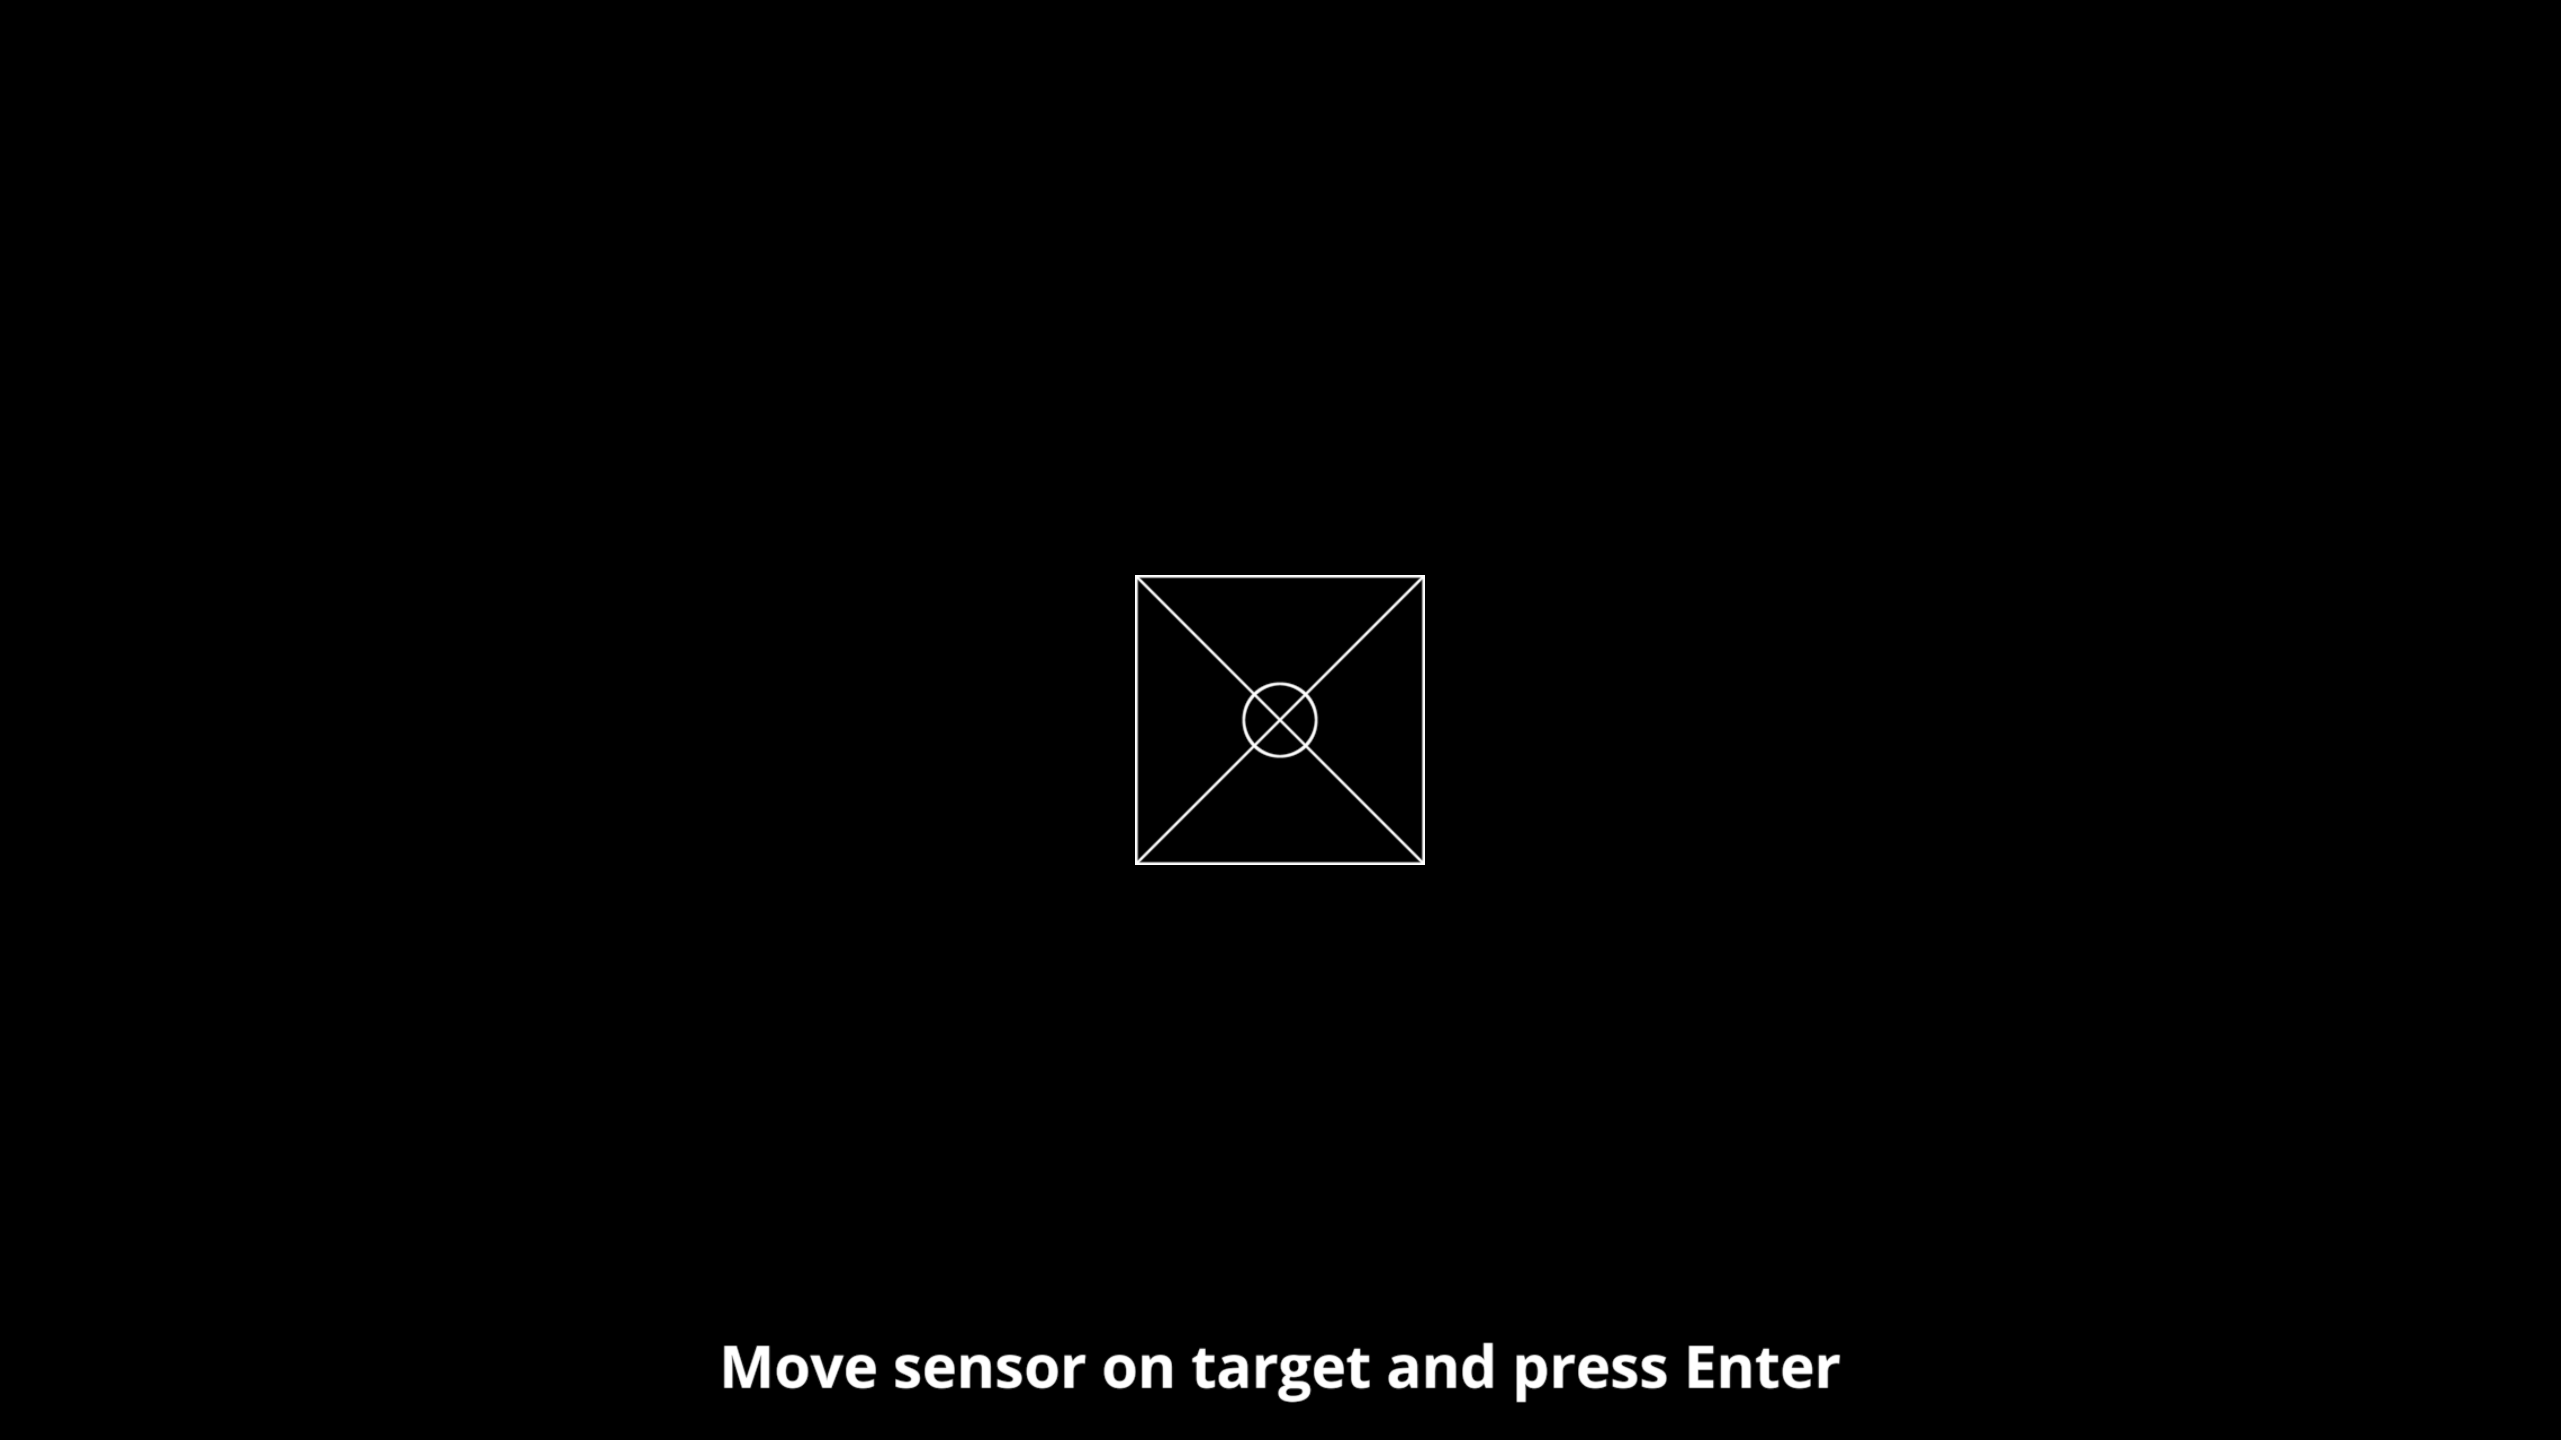
\includegraphics[width=\textwidth]{Applicazione_files/testscreen_example.png}
	\caption{Esempio di output di una schermata di test}
	\label{fig:testscreen_example}
\end{figure}

Entrambe le backend implementano un'interfaccia generica \texttt{ITestScreen}, che definsice le funzionalità minime che un backend deve avere e permette ai test di cambiare backend senza modifiche al codice. L'interfaccia definisce i seguenti metodi pubblici:
\begin{itemize}
	\item \texttt{public int getScreenW()}: ritorna la larghezza dello schermo in pixel
	\item \texttt{public int getScreenH()}: ritorna l'altezza dello schermo in pixel
	\item \texttt{public int getRefreshRate()}: ritorna il refresh rate dello schermo in Hz
	\item \texttt{public boolean setColor(float r, float g, float b)}: imposta il colore dello sfondo con tre valori RGB tra 0 e 1. Ritorna true se il colore nuovo è diverso da quello corrente, altrimenti false
	\item \texttt{public void setTarget(float x, float y, float size, boolean black)}: mostra il target e la scritta ``Move sensor on target and press Enter'' alle coordinate specificate. Le coordinate \texttt{x},\texttt{y} si riferiscono al centro del target e vanno tra 0 e 1, dove 0,0 è l'angolo in alto a sinistra e 1,1 è l'angolo in basso a destra. Impostando \texttt{black} a true, il target e il testo saranno di colore nero, altrimenti saranno bianchi. La dimensione del target è definita come $size*min(W,H)$. Un valore tipico per \texttt{size} è 0.15. Il target è sempre quadrato
	\item \texttt{public void setTargetAbsolute(float x, float y, float size, boolean black)}: analogo a \texttt{setTarget} ma le coordinate sono assolute anziché nel range 0-1
	\item \texttt{public void hideTarget()}: nasconde il target e la scritta precedentemente attivati con \texttt{setTarget} o \texttt{setTargetAbsolute}
	\item \texttt{public void setFlashOnClick(boolean flashOnClick)}: se impostato a \texttt{true}, quando l'applicazione riceve un click genera un flash bianco di 100ms
	\item \texttt{public boolean getFlashOnClick()}: ritorna \texttt{true} se è attualmente attivo il flash in risposta al click (default: disattivato)
	\item \texttt{public void flashColor(float r, float g, float b, double ms)}: genera un flash del colore specificato dai tre valori RGB tra 0 e 1 e della durata specificata
	\item \texttt{public void setFlicker(boolean bkFlicker)}: se impostato a \texttt{true}, il colore dello sfondo si alterna ad ogni fotogramma tra il colore impostato con \texttt{setColor} e il nero
	\item \texttt{public boolean isFlickering()}: ritorna \texttt{true} se è attualmente attivato il flickering (default: disattivato)
	\item \texttt{public void setFakeLoad(long cpuMs, long gpuMs)}: attiva la simulazione di un falso carico sulla CPU e sulla GPU (in millisecondi per frame). Non supportato dalla backend Swing
	\item \texttt{public long getFakeCPULoad()}: ritorna il falso carico attualmente simulato sulla CPU (default: 0)
	\item \texttt{public long getFakeGPULoad()}: ritorna il falso carico attualmente simulato sulla GPU (default: 0)
	\item \texttt{public void close()}: chuiude la schermata di test
	\item \texttt{public void onEnterPressed()}: callback che viene chiamato quando viene premuto il tasto Invio. I test fanno l'override di questo metodo per aggiungere il proprio codice di risposta all'evento. Se non viene fatto l'override, l'evento viene ignorato
	\item \texttt{public void onCancel()}: callback che viene chiamato se viene premuto il tasto Esc per annullare il test. I test fanno l'override di questo metodo per aggiungere il proprio codice di risposta all'evento. Se non viene fatto l'override, l'evento viene ignorato
	\item \texttt{public void onError(Exception e)}: callback che viene chiamato se si verificano errori irreversibili, per esempio in seguito a un crash del driver video. I test fanno l'override di questo metodo per aggiungere il proprio codice di risposta all'evento. Se non viene fatto l'override, il comportamento di default è stampare l'eccezione con il relativo stacktrace e terminare l'applicazione
\end{itemize}

Le due backend hanno due costruttori leggermente diversi:
\begin{itemize}
	\item \texttt{public TestScreenGL(int vsyncMode)}: inizializza la backend OpenGL 2.0 sullo schermo principale. È possibile specificare una modalità per il VSync tra le seguenti costanti definite nella classe stessa:
	\begin{itemize}
		\item \texttt{VSYNC\_OFF}: disabilita il VSync, consentendo le massime prestazioni e il minor ritardo possibile
		\item \texttt{VSYNC\_ON}: attiva il VSync classico con doppio buffering
		\item \texttt{VSYNC\_ON\_ALT}: utilizza il VSync fornito dal compositor del desktop, consentendo all'applicazione di funzionare come se il VSync fosse disattivato (quindi a framerate illimitato) ma evitando comunque il tearing. Non è supportato da tutte le combinazioni hardware e software
	\end{itemize}
	\item \texttt{public TestScreenSwing()}: inizializza la backend Swing sullo schermo principale. Non ci sono impostazioni per questa backend; il VSync (se presente) è fornito dal sistema e non è sotto il controllo dell'applicazione
\end{itemize}

Una volta inizializzata, la backend grafica continua l'esecuzione su un thread parallelo, lasciando al thread principale il compito di coordinare il test interagendo con la backend e con il driver del dispositivo.

Prima di proseguire, è necessario puntualizzare alcune caratteristiche delle backend grafiche:\begin{itemize}
	\item Entrambe le backend vengono eseguite in fullscreen borderless, non in fullscreen esclusivo. Su GNU/Linux, viene disattivato il compositor mentre il test è in esecuzione per evitare che questo penalizzi le performance
	\item La backend OpenGL utilizza lo stesso formato dei pixel e la stessa risoluzione del desktop, tuttavia, a causa di un bug nella libreria LWJGL 3.2.3, l'applicazione potrebbe non dichiarare il supporto HDR/WCG su Windows e quindi mostrare colori errati su display HDR. Questo problema è noto agli sviluppatori di LWJGL e sarà corretto nella release 3.3.0
	\item La backend Swing, poiché utilizza un toolkit grafico pensato per creare interfacce grafiche e non videogiochi, non ha modo di sincronizzarsi con il display, per cui funzioni come \texttt{setFlicker} potrebbero generare un microstuttering che non sarebbe normalmente presente in altre applicazioni grafiche
\end{itemize}

\subsection{Interfaccia standard dei test}
I test implementano tutti un'interfaccia comune, \texttt{ITest}, che definisce alcuni metodi che tutti i test devono implementare:
\begin{itemize}
	\item \texttt{public void begin()}: inizia l'esecuzione del codice del test. A seconda del test, questo può significare l'inizio effettivo del test o semplicemente un'operazione come chiedere all'utente di posizionare il sensore
	\item \texttt{public void cancel()}: richiede al test di terminare il prima possibile. A seconda di come è implementato il test, questo potrebbe terminare immediatamente o richiedere del tempo
	\item \texttt{public void onDone(Map results)}: callback che il codice del test chiama al termine dell'esecuzione del test per riportare i risultati. Il parametro \texttt{results} contiene un insieme di coppie chiave-valore con tutti i risultati ottenuti dal test. Il contenuto esatto è diverso per ogni test
	\item \texttt{public void onError(Exception e)}: callback che il codice del test chiama se si verificano degli errori, come la disconnessione del dispositivo durante il test, o il fallimento dell'analisi. Viene chiamato anche se il test viene annullato manualmente premendo il tasto Esc
\end{itemize}

Ogni test ha il proprio costruttore personalizzato con le relative impostazioni, e può definire altri metodi e callback se necessario.

Vengono inoltre definite due classi di eccezioni speciali: \texttt{IgnorableException} (usata solo internamente per rappresentare eccezioni che non sono degli errori) e \texttt{TestException}, quest'ultima più interessante.

\subsubsection{TestException}
Questa classe è utilizzata per definire alcune condizioni che possono verificarsi durante un test e che ne comportano la terminazione anomala. Questo tipo di eccezione è tipicamente passato al callback \texttt{onError} del test, ma non è necessariamente l'unico tipo di eccezione che quel metodo deve poter gestire (ad esempio, potrebbe ricevere anche eccezioni del backend grafico o del driver del dispositivo).

\paragraph{Costruttori:}\begin{itemize}
	\item \texttt{public TestException(int type)}: crea l'eccezione utilizzando uno dei tipi predefiniti nella classe stessa (\texttt{USER\_ABORT}, \texttt{ANALYSIS\_FAILED}, \texttt{INSUFFICIENT\_CONTRAST}, \texttt{INVALID\_SETTINGS}, \texttt{INCOMPATIBLE\_DEVICE})
	\item \texttt{public TestException(String message)}: crea l'eccezione utilizzando un messaggio personalizzato
\end{itemize}

\paragraph{Metodi pubblici:}\begin{itemize}
	\item \texttt{public int getType()}: ritorna il tipo di eccezione specificata nel costruttore, oppure \texttt{CUSTOM\_ERROR} se è stata inizializzata con un messaggio personalizzato (ottenibile con \texttt{getMessage()})
\end{itemize}

Le sezioni seguenti spiegano nel dettaglio gli algoritmi che sono stati creati per implementare i test e i dati che essi generano. Per una più facile comprensione, vengono omesse tutte le parti irrilevanti dal punto di vista dell'analisi, come la gestione degli errori.

\subsection{Rilevamento PWM e noise}
La classe \texttt{PWMDetectionTest} implementa un test che rileva la presenza di disturbi sul segnale, e in particolar modo la presenza di retroilluminazione PWM, di cui ne misura la frequenza base. Questo è il test più semplice tra quelli implementati.

Il seguente pseudocodice mostra il funzionamento del test.
\lstinputlisting{Applicazione_files/PWMDetectionTest_pseudocode.txt}

Al termine del test, viene chiamato il callback \texttt{onDone} con le seguenti informazioni:\begin{itemize}
	\item \texttt{boolean noisy}: \texttt{true} se c'è qualche tipo di disturbo rilevante sul segnale, altrimenti \texttt{false}
	\item \texttt{double frequency}: la frequenza della PWM rilevata in Hz, oppure 0 se non è stata rilevata alcuna frequenza
	\item \texttt{int[] raw}: array contenente i sample catturati dal sensore nel dominio temporale come interi tra 0 e 1023
	\item \texttt{double sampleRate}: il sample rate dell'array \texttt{raw}, così da poter calcolare il timestamp a cui corrisponde ogni sample
\end{itemize}

\subsection{Input lag (test automatico)}
La classe \texttt{InputLagTest} implementa il test che rileva la latenza totale del sistema, ossia il tempo che passa tra un click del mouse e la visualizzazione del risultato sul display.

Il test utilizza la generazione automatica dei click del dispositivo OpenLDAT per generare dei click che l'applicazione riceve e a cui risponde generando un flash bianco sullo schermo, che viene catturato dal sensore di luminosità. Il test esegue questo processo per alcuni secondi, poi analizza i dati per associare ogni flash al click corrispondente.

Il test ha alcuni parametri in input, da passare al costruttore:\begin{itemize}
	\item \texttt{int durationMs}: durata del test in millisecondi (si consiglia almeno 20000)
	\item \texttt{int vsyncMode}: permette di scegliere una delle modalità di VSync del backend grafico OpenGL. Ignorato se si usa il backend Swing
	\item \texttt{long fakeCPULoadMs}: simula un carico sulla CPU durante il test, espresso in millisecondi per frame. Ignorato se si usa il backend Swing
	\item \texttt{long fakeGPULoadMs}: simula un carico sulla GPU durante il test, espresso in millisecondi per frame. Ignorato se si usa il backend Swing
\end{itemize}

La principale difficoltà che questo test deve saper affrontare è la presenza di retroilluminazione PWM, poiché in questo caso il segnale catturato potrebbe contenere più transizioni dal nero al bianco per ogni click. I grafici in figura \ref{fig:inputLagTest_example} mostrano come potrebbero presentarsi i segnali in questa situazione.
\begin{figure}[H]
	\centering
	\begin{tikzpicture}
		\begin{axis}[name=Segnale, xmin=0,xmax=0.5,ymin=0,ymax=1023,width=.45\textwidth,xlabel=Tempo (s),ylabel=Valore,xticklabel style={/pgf/number format/fixed}]
			\addplot[black] file{Applicazione_files/inputLagTest_example_light.txt};
			\addplot[blue] file{Applicazione_files/inputLagTest_example_click.txt};
		\end{axis}
	\end{tikzpicture}
	\begin{tikzpicture}
		\begin{axis}[name=Segnale, xmin=0,xmax=0.5,ymin=0,ymax=1023,width=.45\textwidth,xlabel=Tempo (s),ylabel=Valore,xticklabel style={/pgf/number format/fixed}]
			\addplot[black] file{Applicazione_files/inputLagTest_example_lightpwm.txt};
			\addplot[blue] file{Applicazione_files/inputLagTest_example_click.txt};
		\end{axis}
	\end{tikzpicture}
	\caption{Segnale senza PWM (sinistra) e segnale con PWM (destra). I picchi blu indicano i click. (Simulato, non è una cattura reale)}
	\label{fig:inputLagTest_example}
\end{figure}

Il seguente pseudocodice mostra il funzionamento del test.
\lstinputlisting{Applicazione_files/InputLagTest_pseudocode.txt}

Al termine del test, viene chiamato il callback \texttt{onDone} con le seguenti informazioni:\begin{itemize}
	\item \texttt{Double[] times}: array contenente le latenze in millisecondi misurate tra ogni coppia di click-transizione
	\item \texttt{double percentileL}: il 33-esimo percentile delle latenze misurate
	\item \texttt{double percentile50}: il 50-esimo percentile delle latenze misurate. Questo è il dato a cui siamo più interessati
	\item \texttt{double percentileL}: il 66-esimo percentile delle latenze misurate
	\item \texttt{Double[] distribution}: distribuzione dei tempi di latenza misurati
\end{itemize}

Su molti display è possibile osservare che il risultato ha un pattern a dente di sega causato dal fatto che i click non sono in alcun modo sincronizzati con il display, per cui se un click arriva dopo che la parte di immagine dove si trova il sensore è già stata disegnata (VSync off) oppure dopo l'intervallo di VBlank (VSync on), il sensore potrà vederlo solo nel fotogramma successivo.

\subsection{Rilevamento del microstuttering}
La classe \texttt{StutteringDetectionTest} implementa il test di rilevazione del microstuttering. Per microstuttering si intende la presenza di fotogrammi persi o duplicati, che causano dei visibili scatti nelle immagini in movimento.

Il test visualizza fotogrammi alternati bianchi e neri per alcuni secondi mentre cattura il segnale ottenuto con il sensore di luminosità, il segnale viene poi analizzato per rilevare le transizioni dal nero al bianco e trovare deviazioni nei tempi di queste transizioni. Normalmente, tra ogni coppia di transizioni successive dal nero-bianco passano circa $2*\frac{1000}{RefreshRate}$ millisecondi, ma se un fotogramma (bianco o nero) viene duplicato o perso, si noterà un picco in uno di questi tempi, e questo consente di rilevare il microstuttering.\\
Il grafico in figura \ref{fig:stutteringDetectionTest_example} mostra come potrebbe presentarsi un segnale catturato durante il test: il fotogramma nero che dovrebbe essere presente tra 0.1 e 0.15s è stato perso, e con esso una transizione, e questo viene rilevato dall'algoritmo alla transizione successiva.

In presenza di rumore, in particolar modo retroilluminazione PWM, viene utilizzato il filtro \texttt{RunningAverageSmoothingFilter} per ridurlo notevolmente così che non causi problemi all'analisi.

\begin{figure}[H]
	\centering
	\begin{tikzpicture}
		\begin{axis}[name=Segnale, xmin=0,xmax=0.2,ymin=0,ymax=1023,width=.5\textwidth,xlabel=Tempo (s),ylabel=Valore,xticklabel style={/pgf/number format/fixed}]
			\addplot[black] file{Applicazione_files/stuttering_example.txt};
		\end{axis}
	\end{tikzpicture}
	\caption{Segnale catturato in presenza di microstuttering. (Simulato, non è una cattura reale)}
	\label{fig:stutteringDetectionTest_example}
\end{figure}

Il test accetta un parametro in input, da passare al costruttore:\begin{itemize}
	\item \texttt{int durationMs}: durata del test in millisecondi. Si consiglia 5-10 secondi, poiché il flickering eccessivo potrebbe danneggiare alcuni display
\end{itemize}

Il seguente pseudocodice mostra il funzionamento del test.
\lstinputlisting{Applicazione_files/StutteringDetectionTest_pseudocode.txt}

Al termine del test, viene chiamato il callback \texttt{onDone} con le seguenti informazioni:\begin{itemize}
	\item \texttt{boolean flickeringDetected}: \texttt{true} se il test ha rilevato rumori, come retroilluminazione PWM, che potrebbero ridurre l'accuratezza del test
	\item \texttt{Double[] frameTimes}: array contenente i tempi in millisecondi tra ogni coppia di transizioni nero-bianco successive
	\item \texttt{double stutteringThreshold}: soglia di millisecondi sopra di cui il test considera un tempo stuttering
	\item \texttt{int stutters}: numero di stutter rilevati durante il test
\end{itemize}

\subsection{Tempi di risposta dei pixel}
La classe \texttt{PixelResponseTimeTest} implementa il test che misura i tempi di risposta dei pixel, ossia il tempo che i pixel impiegano per passare tra un livello di luminosità e un altro. L'output del test è una tabella contenente il tempo di transizione tra ogni coppia di valori di luminosità testati.

Per ogni coppia di livelli di luminosità, il test esegue le seguenti operazioni:\begin{itemize}
	\item Cattura il livello di luminosità iniziale
	\item Esegui la transizione mentre viene catturata la luminosità
	\item Cattura il livello di luminosità finale
	\item Analizza il segnale catturato per determinare il tempo di transizione
\end{itemize}

Una tipica transizione tra livelli di luminosità si presenta come in figura \ref{fig:pixelResponseTime_example1}. Il test deve saper gestire, oltre all'eventuale presenza di retroilluminazione PWM, anche la presenza di picchi causati dall'overdrive dei pixel, se attivo, come in figura \ref{fig:pixelResponseTime_example2}. L'overdrive dei pixel sarà approfondito nella sezione successiva dedicata al relativo test.

Tradizionalmente i tempi di transizione erano misurati come il tempo richiesto per passare dal nero al bianco e viceversa, ma dal 2005 lo standard VESA\cite{vesa_measurementstd} stabilisce che i tempi di transizione dei pixel vanno misurati come l'intervallo di tempo richiesto per eseguire la parte di transizione tra il 10\% e il 90\% tra due sfumature di grigio (da cui il nome GtG, Gray-to-Gray). Un metodo alternativo, non implementato in questo test, è MPRT\cite{mprt}, che si concentra sulla percezione del motion blur. La maggior parte dei produttori di display, purtroppo, soprattutto nel settore non professionale, si inventa il proprio metodo di misurazione per poter dichiarare tempi di risposta di 1ms. Questo test usa lo stesso metodo dello standard VESA per il calcolo del tempo di transizione, ossia misura il tempo per completare la transizione dal 10\% al 90\%, ma anziché generare un singolo valore, genera una tabella di tempi di transizione tra molte sfumature di grigio.

Display dotati di retroilluminazione PWM, black frame insertion, o altri tipi di strobing possono fare uso dei lampeggi per cercare di nascondere i tempi di transizione visibili. Il test in questo caso è in grado solo di misurare la parte visibile della transizione.

\begin{figure}[H]
	\centering
	\begin{tikzpicture}
		\begin{axis}[name=Segnale, xmin=0,xmax=0.3,ymin=0,ymax=1023,width=.45\textwidth,xlabel=Tempo (s),ylabel=Valore,xticklabel style={/pgf/number format/fixed}]
			\addplot[black] file{Applicazione_files/pixelResponseTime_example1_normal.txt};
		\end{axis}
	\end{tikzpicture}
	\begin{tikzpicture}
		\begin{axis}[name=Segnale, xmin=0,xmax=0.3,ymin=0,ymax=1023,width=.45\textwidth,xlabel=Tempo (s),ylabel=Valore,xticklabel style={/pgf/number format/fixed}]
			\addplot[black] file{Applicazione_files/pixelResponseTime_example1_pwm.txt};
		\end{axis}
	\end{tikzpicture}
	\caption{Segnale senza PWM (sinistra) e segnale con PWM (destra). (Simulato, non è una cattura reale)}
	\label{fig:pixelResponseTime_example1}
\end{figure}

\begin{figure}[H]
	\centering
	\begin{tikzpicture}
		\begin{axis}[name=Segnale, xmin=0,xmax=0.3,ymin=0,ymax=1023,width=.45\textwidth,xlabel=Tempo (s),ylabel=Valore,xticklabel style={/pgf/number format/fixed}]
			\addplot[black] file{Applicazione_files/pixelResponseTime_example2_normal.txt};
		\end{axis}
	\end{tikzpicture}
	\begin{tikzpicture}
		\begin{axis}[name=Segnale, xmin=0,xmax=0.3,ymin=0,ymax=1023,width=.45\textwidth,xlabel=Tempo (s),ylabel=Valore,xticklabel style={/pgf/number format/fixed}]
			\addplot[black] file{Applicazione_files/pixelResponseTime_example2_pwm.txt};
		\end{axis}
	\end{tikzpicture}
	\caption{Segnale in presenza di overdrive senza PWM (sinistra) e con PWM (destra). (Simulato, non è una cattura reale)}
	\label{fig:pixelResponseTime_example2}
\end{figure}

Il test ha alcuni parametri in input, da passare al costruttore:\begin{itemize}
	\item \texttt{int step}: dimensione del passo tra un livello di luminosità e un altro, sul range 0-255. Si consigliano 16, 32 o 64. Valori più bassi rendono il test più lungo, ma testano più transizioni. (Nota: il valore è espresso nel range 0-255 solo per comodità, internamente vengono convertiti in float nel range 0-1 indipendenti dal formato dei pixel)
	\item \texttt{float th1, float th2}: le soglie di inizio e fine transizione, nel range 0-1. Per lo standard VESA sono 0.1 e 0.9 rispettivamente
\end{itemize}

Il seguente pseudocodice mostra il funzionamento del test.
\lstinputlisting{Applicazione_files/PixelResponseTimeTest_pseudocode.txt}

Al termine del test, viene chiamato il callback \texttt{onDone} con le seguenti informazioni:\begin{itemize}
	\item \texttt{int[] steps}: array contenente i livelli di luminosità usati nel test come interi nel range 0-255
	\item \texttt{boolean flickeringDetected}: true se il test ha rilevato rumori, come retroilluminazione PWM, che potrebbero ridurre l'accuratezza del test
	\item Molti elementi \texttt{double tFrom>To}: i tempi di risposta in millisecondi misurati nella transizione da \texttt{From} a \texttt{To}, dove \texttt{From} e \texttt{To} sono elementi dell'array steps. Sono omessi gli elementi in cui \texttt{From=To}, il cui valore è da considerarsi 0
\end{itemize}

\subsection{Overdrive dei pixel}
La classe \texttt{PixelOverdriveTest} implementa il test che misura l'errore massimo che viene raggiunto dal pixel durante la transizione tra due livelli di luminosità. Normalmente, questo errore è praticamente nullo, ma negli ultimi anni molti display hanno implementato una tecnica comunemente nota come overdrive, che velocizza la transizione da un livello A a un livello B spingendo brevemente il pixel oltre il livello B. A livelli bassi, questa tecnica velocizza notevolmente le transizioni senza causare un notevole overshoot/undershoot, ma ai livelli più alti (e i produttori solitamente misurano i tempi di transizione utilizzando il livello massimo) causa inverse ghosting, ossia degli artefatti molto visibili sotto forma di scie nere o bianche attorno agli oggetti in movimento, come in figura \ref{fig:overdrive_ufotest}.
\begin{figure}[H]
	\centering
	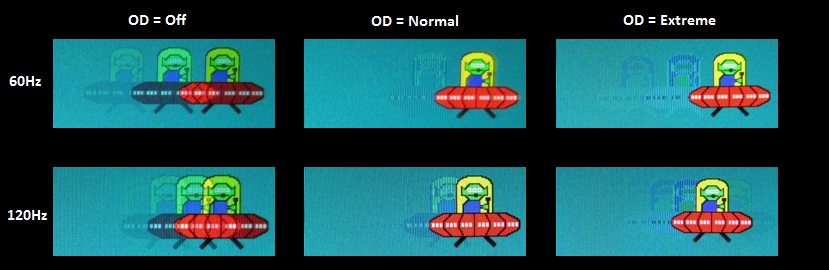
\includegraphics[width=\textwidth]{Applicazione_files/overdrive_ufotest.png}
	\caption{Esempio di artefatti generati dall'overdrive dei pixel (da anandtech.com)}
	\label{fig:overdrive_ufotest}
\end{figure}

Non esiste uno standard per la misurazione dell'overdrive, quindi in questo test vengono proposti due metodi:\begin{itemize}
	\item \texttt{Assoluto}: considera l'errore sull'intero range di luminosità del display. Ad esempio, se durante una transizione da 16 a 32 si raggiunge un livello di 48, l'overshoot è $\frac{48-32}{255}=6.25\%$ . Questo è il metodo consigliato
	\item \texttt{Relativo}: considera l'errore relativo al range di luminosità che la transizione deve percorrere. Ad esempio, se durante una transizione da 16 a 32 si raggiunge un livello di 48, l'overshoot è  $\frac{48-32}{32-16}=50\%$. Questo metodo tende a sovrastimare molto i risultati su transizioni piccole, per cui è quindi generalmente sconsigliato
\end{itemize}

Tra tutti i test implementati nell'applicazione, questo è quello che soffre di più della presenza di rumore, soprattutto retroilluminazione PWM, poiché il test deve misurare delle caratteristiche nel segnale che potrebbero avere una frequenza molto alta. La figura \ref{fig:pixelOverdriveTest_example1} mostra come il segnale potrebbe presentarsi, prima in modo pulito, e poi in presenza di PWM. Si può osseravare fin da subito che se la frequenza della retroilluminazione PWM è troppo bassa, è completamente impossibile ricostruire il segnale originale, per cui in presenza di retroilluminazione PWM il test tende a sottostimare significativamente l'errore.

\begin{figure}[H]
	\centering
	\begin{tikzpicture}
		\begin{axis}[name=Segnale, xmin=0,xmax=0.3,ymin=0,ymax=1023,width=.45\textwidth,xlabel=Tempo (s),ylabel=Valore,xticklabel style={/pgf/number format/fixed}]
			\addplot[black] file{Applicazione_files/pixelOverdriveTest_example_normal.txt};
		\end{axis}
	\end{tikzpicture}
	\begin{tikzpicture}
		\begin{axis}[name=Segnale, xmin=0,xmax=0.3,ymin=0,ymax=1023,width=.45\textwidth,xlabel=Tempo (s),ylabel=Valore,xticklabel style={/pgf/number format/fixed}]
			\addplot[black] file{Applicazione_files/pixelOverdriveTest_example_pwm.txt};
		\end{axis}
	\end{tikzpicture}
	\caption{Segnale senza PWM (sinistra) e segnale con PWM (destra). (Simulato, non è una cattura reale)}
	\label{fig:pixelOverdriveTest_example1}
\end{figure}

Il grafico in figura \ref{fig:pixelOverdriveTest_example2} mostra il segnale ricostruito dall'algoritmo osservando i picchi in presenza di retroilluminazione PWM. Il segnale ricostruito in questo caso ha comunque un picco in corrispondenza dell'overshoot, ma è più piccolo e potrebbe essere addirittura assente, per cui non può essere misurato accuratamente dall'applicazione. Le transizioni dal chiaro allo scuro sono più affette da questo problema rispetto a quelle dallo scuro al chiaro.

\begin{figure}[H]
	\centering
	\begin{tikzpicture}
		\begin{axis}[name=Segnale, xmin=0,xmax=0.5,ymin=0,ymax=1023,width=.7\textwidth,xlabel=Tempo (s),ylabel=Valore,xticklabel style={/pgf/number format/fixed}]
			\addplot[lightgray] file{Applicazione_files/pixelOverdriveTest_example_pwm.txt};
			\addplot[red] file{Applicazione_files/pixelOverdriveTest_example_phf.txt};
		\end{axis}
	\end{tikzpicture}
	\caption{Segnale con PWM (grigio), Segnale filtrato con PeakHoldFilter (rosso). (Simulato, non è una cattura reale)}
	\label{fig:pixelOverdriveTest_example2}
\end{figure}

Il test ha alcuni parametri in input, da passare al costruttore:\begin{itemize}
	\item \texttt{int step}: dimensione del passo tra un livello di luminosità e un altro, sul range 0-255. Si consigliano 16, 32 o 64. Valori più bassi rendono il test più lungo, ma testano più transizioni. (Nota: il valore è espresso nel range 0-255 solo per comodità, internamente vengono convertiti in float nel range 0-1 indipendenti dal formato dei pixel)
	\item \texttt{boolean skipTo0And255}: velocizza il test saltando le transizioni verso 0 e 255, poiché normalmente la luminosità non può scendere sotto il livello di nero, nè sopra il livello di bianco
	\item \texttt{int method}: permette di scegliere tra i due metodi di misurazione (\texttt{METHOD\_ABSOLUTE} o \texttt{METHOD\_RELATIVE})
\end{itemize}

Il seguente pseudocodice mostra il funzionamento del test.
\lstinputlisting{Applicazione_files/PixelOverdriveTest_pseudocode.txt}

Al termine del test, viene chiamato il callback \texttt{onDone} con le seguenti informazioni:\begin{itemize}
	\item \texttt{int[] steps}: array contenente i livelli di luminosità usati nel test come interi nel range 0-255
	\item \texttt{boolean flickeringDetected}: true se il test ha rilevato rumori, come retroilluminazione PWM, che potrebbero ridurre l'accuratezza del test
	\item Molti elementi \texttt{double eFrom>To}: la percentuale di overshoot/undershoot misurata nella transizione da \texttt{From} a \texttt{To}, dove \texttt{From} e \texttt{To} sono elementi dell'array steps. Sono omessi gli elementi in cui \texttt{From=To}, il cui valore è da considerarsi 0
\end{itemize}

\subsection{Input lag (test interattivo)}
La classe \texttt{InteractiveInputLagTest} implementa un test della latenza toatle del sistema, ma a differenza di quello discusso precedentemente, questa è una versione interattiva anziché automatica. A differenza del test automatico, questo test non utilizza affatto un backend grafico: si limita a ricevere i dati dal dispositivo e analizzarli mentre li riceve. Questo test consente di testare il ritardo di input di applicazioni grafiche esterne, in particolar modo videogiochi, in esecuzione sulla stessa macchina o addirittura su una macchina separata.

Il funzionamento del test può essere descritto in modo intuitivo dall'automa a stati finiti in figura \ref{fig:interactiveInputLagTest_fsm}.

\begin{figure}[H]
	\centering
	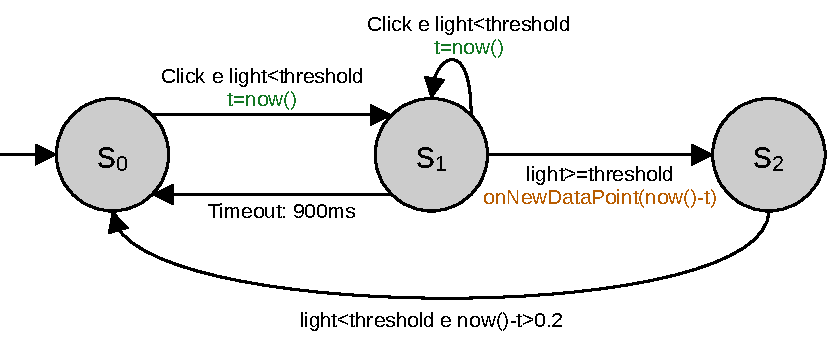
\includegraphics[width=.8\textwidth]{Applicazione_files/interactiveInputLagTest_fsm.pdf}
	\caption{Funzionamento di \texttt{InteractiveInputLagTest}. Le etichette verdi indicano operazioni su variabili, quelle rosse dei callback}
	\label{fig:interactiveInputLagTest_fsm}
\end{figure}

I tre stati hanno i seguenti significati:\begin{itemize}
	\item \textbf{$S_0$}: In attesa del click
	\item \textbf{$S_1$}: Click ricevuto, in attesa del flash
	\item \textbf{$S_2$}: Flash ricevuto, in attesa che finisca
\end{itemize}

All'inizializzazione, è possibile passare al costruttuore due istanze di \texttt{IBuffer}, su cui il test scriverà i valori catturati dal sensore di luminosità e dal pulsante, così che sia possibile visualizzarli nell'interfaccia grafica.

Oltre ai metodi dell'interfaccia standard \texttt{ITest}, questa classe implementa anche i seguenti metodi pubblici: \begin{itemize}
	\item \texttt{public abstract void onNewDataPoint(double delay)}: callback che viene chiamato quando è disponibile un nuovo dato sulla latenza. Il parametro \texttt{delay} contiene il tempo in millisecondi trascorso tra il click e il flash. Attenzione: questo metodo deve terminare il prima possibile per evitare di rallentare il campionamento
	\item \texttt{public void setThreshold(int threshold)}: permette di impostare la soglia di rilevazione del flash come intero tra 0 e 1023
	\item \texttt{public int getThreshold()}: ritorna la soglia di rilevazione del flash corrente come intero tra 0 e 1023. Il valore di default è 100
	\item \texttt{public void setSensitivity(byte sensitivity)}: imposta la sensibilità del sensore tra i quattro valori possibili (0=minima, 3=massima)
	\item \texttt{public byte getSensitivity()}: ritorna la sensibilità attuale del sensore. Il valore di default è 2
	\item \texttt{public void setAutoFire(boolean autoFire)}: permette di attivare o disattivare la generazione automatica dei click anziché utilizzare il pulsante esterno
	\item \texttt{public boolean getAutoFire()}: ritorna \texttt{true} se il dispositivo sta generando i click, false se li riceve dal pulsante esterno. Di default li riceve dall'esterno. Il valore di default è \texttt{false}
	\item \texttt{public byte getState()}: ritorna lo stato attuale dell'automa in figura \ref{fig:interactiveInputLagTest_fsm}
\end{itemize}

Il test prosegue indefinitamente fino a quando non viene terminato manualmente dall'utente chiamando il metodo \texttt{onCancel}. Il callback \texttt{onDone} viene comunque chiamato alla terminazione ma non gli viene passato nessun dato.

Il test può essere utilizzato in due modi:\begin{itemize}
	\item \textbf{Sulla stessa macchina}: in questo caso è sufficiente avviare il test e attivare la generazione automatica dei click. Il dispositivo genera click a una frequenza di circa 1 click al secondo, e posizionando il dispositivo in corrispondenza del muzzle flash di un'arma o qualche altro elemento del gioco che genera un flash in risposta ai click, è possibile misurare quanto tempo passa tra un click e la generazione del flash
	\item \textbf{Su una macchina separata}: si avvia il test utilizzando come fonte dei click il pulsante esterno, si collegano i pin del pulsante esterno ad un mouse o appositamente modificato come spiegato nel capitolo precedente sull'hardware, si posiziona il sensore sul display della macchina da testare come nel caso precedente, e il test misura il tempo che passa tra la pressione del pulsante e la generazione del flash. Si consiglia di far passare almeno mezzo secondo tra un click e l'altro
\end{itemize}

Durante il test, è possibile regolare manualmente la soglia di rilevazione del flash e la sensibilità del sensore. La soglia di rilevazione deve essere impostata il più bassa possibile, ma alta abbastanza da non attivarsi accidentalmente. Per risultati migliori, è consigliabile posizionarsi in un'area scura e utilizzare un'arma o un altro elemento del gioco che genera un flash immediatamente quando viene premuto il pulsante, senza eseguire un'animazione prima.

\subsection{Light to sound}
La classe \texttt{InteractiveLightToSound} implementa un altro test interattivo, che consente di ascoltare il segnale catturato dal dispositivo. Pur non producendo alcun risultato, questo test consente di puntare il dispositivo verso lampadine o altri dispositivi luminosi e sentire immediatamente se la luce è stabile o se ha disturbi. Nel caso delle lampadine, i disturbi sono principalmente causati da un circuito di rettificazione e filtraggio dell'alimentazione inadeguato che causa un flickering a 50 o 100Hz più o meno visibile, che a lungo termine può affaticare la vista.\\
Il test è implementato utilizzando le classi dell'audio \texttt{javax.sound.sampled}. Durante il test, è possibile variare il volume dell'output e la sensibilità del sensore.

Oltre ai metodi dell'interfaccia standard \texttt{ITest}, questa classe implementa anche i seguenti metodi pubblici: \begin{itemize}
	\item \texttt{public void setSensitivity(byte sensitivity)}: imposta la sensibilità del sensore tra i quattro valori possibili (0=minima, 3=massima)
	\item \texttt{public byte getSensitivity()}: ritorna la sensibilità attuale del sensore. Il valore di default è 2
	\item \texttt{public void setVolume(int volume)}: imposta il volume dell'output come un numero tra 0 e 1
	\item \texttt{public float getVolume()}: ritorna il volume corrente. Il valore di default è 1
	\item \texttt{public double getSampleRate()}: ritorna il sample rate in Hz
	\item \texttt{public IBuffer getChartBuffer()}: ritorna un'istanza di \texttt{CircularBuffer} contenente l'ultimo mezzo secondo di audio, così che sia possibile visualizzarlo nell'interfaccia grafica. Il contenuto del buffer ritornato è sempre aggiornato, non è necessario riottenerlo ogni volta che serve
	\item \texttt{public double getStrongestFrequency(double from, double to)}: ritorna la frequenza in Hz più forte nel range specificato, oppure -1 se non ce ne sono o sono troppo deboli per essere rilevanti
\end{itemize}

Il test prosegue indefinitamente fino a quando non viene terminato manualmente dall'utente chiamando il metodo \texttt{onCancel}. Il callback \texttt{onDone} viene comunque chiamato alla terminazione ma non gli viene passato nessun dato.

%RIMOSSO PER DUBBIA UTILITÀ, meglio metterlo nella documentazione
%\subsection{Template per test automatici}
%Il seguente listato mostra il codice minimo per eseguire un test automatico utilizzando i backend grafici forniti e un thread eseguire per il test.
%
%\lstinputlisting[language=Java]{Applicazione_files/TestExample.java}
%
Questo conclude la sezione dedicata all'implementazione dei test.

\section{Interfaccia grafica}
Questa sezione è dedicata all'interfaccia grafica dell'applicazione OpenLDAT, implementata nel package \texttt{com.dosse.openldat.ui}.

L'interfaccia è stata sviluppata utilizzando le librerie Swing di Java SE con alcuni accorgimenti per supportare i display con DPI alti, e permette di avviare i test e visualizzarne i risultati in maniera semplice e intuitiva. Non c'è nulla di particolarmente interessante dal punto di vista tecnico nell'implementazione della GUI, per cui questa sezione si concentra principalmente sulle funzionalità e l'utilizzo dell'interfaccia grafica.

Attualmente non sono implementate localizzazioni, l'interfaccia è disponibile solo in lingua Inglese.

L'interfaccia è pensata per essere utilizzata con un mouse, ma è presente un supporto limitato per i touchscreen e la navigazione da tastiera.

\subsection{Selezione del dispositivo}
All'avvio dell'applicazione viene scansionato il PC per trovare dispositivi OpenLDAT connessi. Se viene trovato più di un dispositivo, viene mostrata una schermata di selezione come quella in figura \ref{fig:gui_deviceSelector} da cui è possibile distinguerli in base alla porta a cui sono collegati. Se c'è un solo dispositivo questa schermata viene saltata.

\begin{figure}[h]
	\centering
	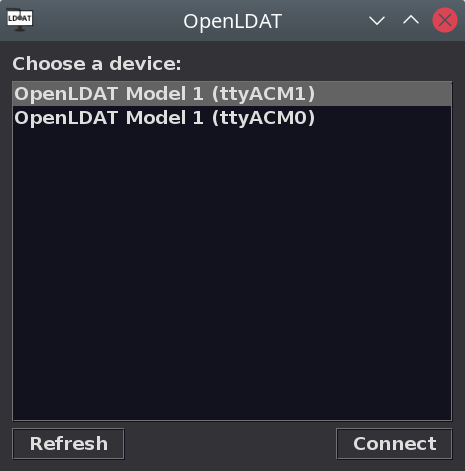
\includegraphics[width=.5\textwidth]{Applicazione_files/gui_deviceSelector.png}
	\caption{Selezione del dispositivo}
	\label{fig:gui_deviceSelector}
\end{figure}

Premendo il pulsante Connect si avvia l'applicazione utilizzando il dispositivo selezionato, premendo Refresh è possibile rieseguire la scansione.

\subsection{Menu principale}
Dopo la selezione del dispositivo, viene visualizzato il menu principale dell'applicazione come in figura \ref{fig:gui_mainMenu2}. Questa schermata è divisa in due parti: a sinistra sono elencati tutti i test e le funzioni dell'applicazione, sulla destra è presente un manuale che mostra informazioni sul test selezionato e il pulsante per avviarlo. Le pagine del manuale mostrato sulla destra sono memorizzate come dei file HTML nella cartella \texttt{manual} all'interno del package della GUI.

\begin{figure}[h]
	\centering
	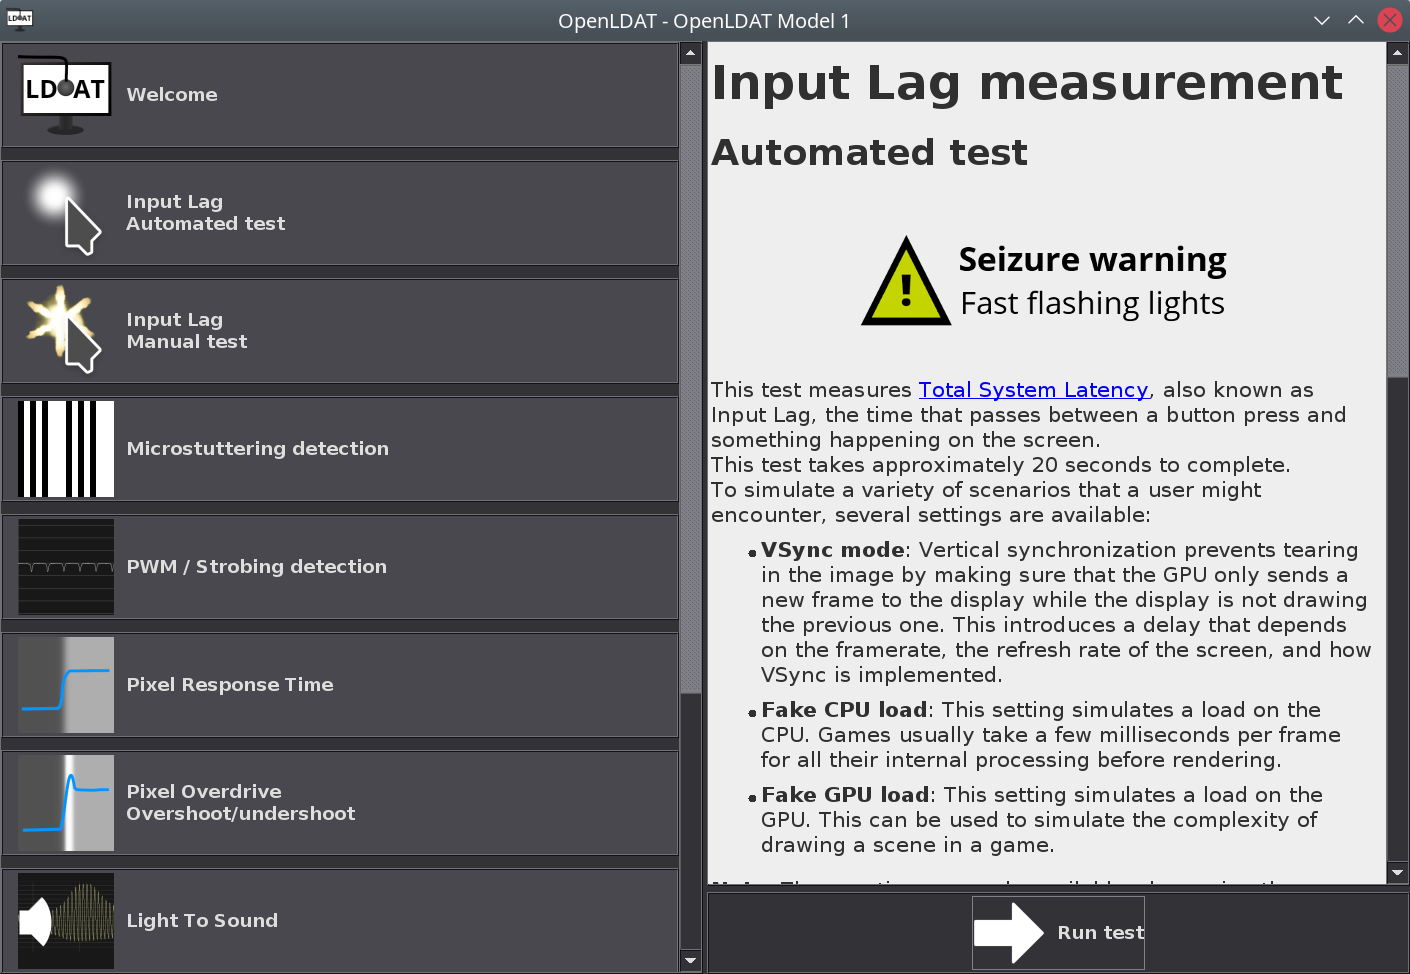
\includegraphics[width=\textwidth]{Applicazione_files/gui_mainMenu2.png}
	\caption{Menu principale con un test selezionato}
	\label{fig:gui_mainMenu2}
\end{figure}

Il menu principale fornisce accesso alle seguenti funzioni:\begin{itemize}
	\item \textbf{Welcome}: mostra una schermata di benvenuto con alcuni suggerimenti generali per l'utilizzo corretto dei test
	\item \textbf{Input Lag (Automated test)}: esegue il test automatico del ritardo di input
	\item \textbf{Input Lag (Manual test)}: esegue il test interattivo del ritardo di input
	\item \textbf{Microstuttering detection}: esegue il test di rilevamento del microstuttering
	\item \textbf{PWM/Strobing test}: esegue il test di rilevamento PWM e altri rumori
	\item \textbf{Pixel Response Time}: esegue il test che misura il tempo di risposta dei pixel tra diverse sfumature di grigio
	\item \textbf{Pixel Overdrive (Overshoot/Undershoot)}: esegue il test che misura l'errore di transizione causato dall'overdrive dei pixel
	\item \textbf{Light To Sound}: avvia la modalità Light To Sound, per ascoltare i dati catturati dal sensore di luminosità
	\item \textbf{Driver test}: fornsice accesso a un pannello da cui è possibile testare tutte le funzioni del dispositivo, del driver, e dell'elaborazione di base
	\item \textbf{Advanced settings}: permette di cambiare alcune impostazioni dell'applicazione che normalmente sono determinate automaticamente
	\item \textbf{About OpenLDAT}: mostra informazioni sull'applicazione
\end{itemize}

\subsection{Test automatici}
I test automatici seguono tutti i seguenti passi quando vengono avviati:\begin{itemize}
	\item Se il test ha dei parametri configurabili, mostra una schermata di configurazione
	\item Esegui il test
	\item Mostra una schermata con i risultati
	\item Torna al menu principale
\end{itemize}

\subsubsection{Input lag (test automatico)}
Questo test ha dei parametri che possono essere configurati, mostrati in figura \ref{fig:gui_inputlag_settings}:\begin{itemize}
	\item \textbf{VSync mode}: permette di attivare o disattivare il VSync
	\item \textbf{Fake CPU load}: simula la presenza di carico sulla CPU durante l'esecuzione del test. Il carico è espresso in millisecondi per frame
	\item \textbf{Fake GPU load}: simula la presenza di carico sulla GPU durante l'esecuzione del test. Il carico è espresso in millisecondi per frame
	\item \textbf{Test duration}: permette di selezionare la durata del test tra 20 secondi, 1 minuto (default), 2 minuti o 5 minuti. Test più lunghi garantiscono risultati più accurati
\end{itemize}

Al termine del test, viene visualizzata una schermata con i risultati come in figura \ref{fig:gui_inputlag_results}. Da quì è possibile salvarli su un file importabile in un foglio di calcolo oppure tornare al menu principale.

\begin{figure}[H]
	\centering
	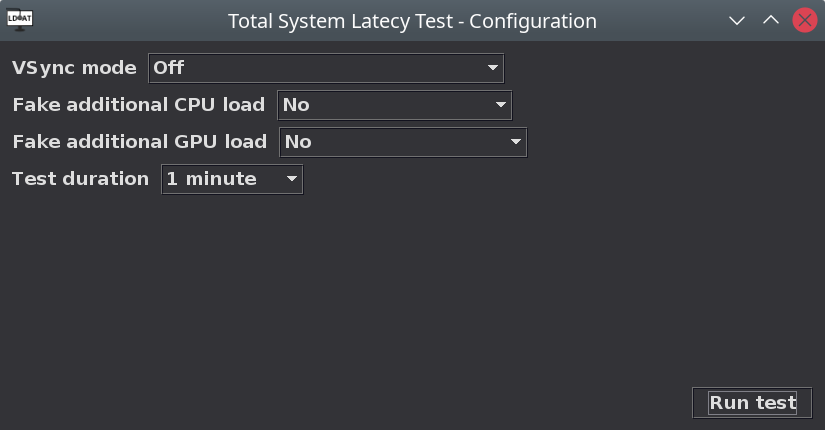
\includegraphics[width=.8\textwidth]{Applicazione_files/gui_inputlag_settings.png}
	\caption{Input lag: impostazioni del test}
	\label{fig:gui_inputlag_settings}
\end{figure}

\begin{figure}[H]
	\centering
	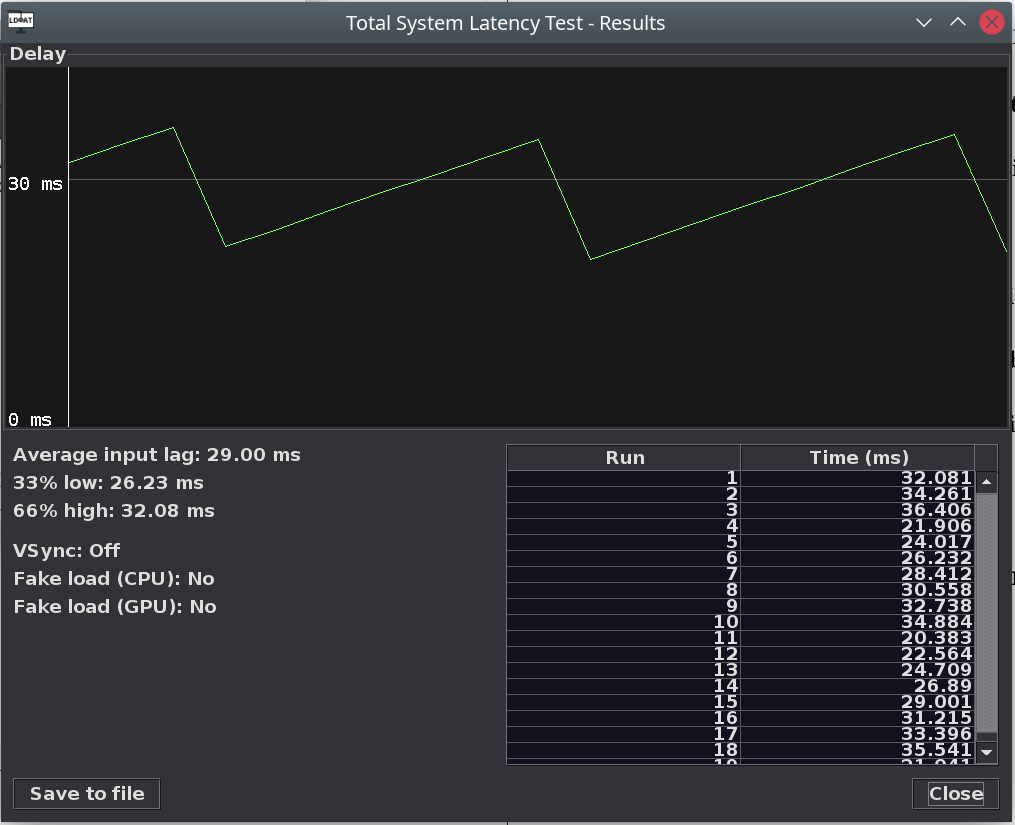
\includegraphics[width=\textwidth]{Applicazione_files/gui_inputlag_results.png}
	\caption{Input lag: risultati del test}
	\label{fig:gui_inputlag_results}
\end{figure}

\subsubsection{Rilevamento del microstuttering}
Questo test non ha parametri da configurare, per cui viene eseguito immediatamente. Al termine viene mostrata una schermata con i risultati come in figura \ref{fig:gui_microstuttering_results}. Da quì è possibile salvarli su un file importabile in un foglio di calcolo oppure tornare al menu principale. La presenza di picchi sopra la linea rossa nel grafico indica la presenza di microstuttering.

Nota: è stato osservato che su alcune piattaforme, il backend Swing, non essendo in grado di sincronizzarsi con il display, può generare esso stesso microstuttering; per questo motivo, al fine di evitare di fornire dati potenzialmente errati, è stato scelto di far funzionare questo test solo con il backend OpenGL. Il codice del test supporta entrambi i backend, la restrizione è presente solo nel codice della GUI che avvia il test.

\begin{figure}[H]
	\centering
	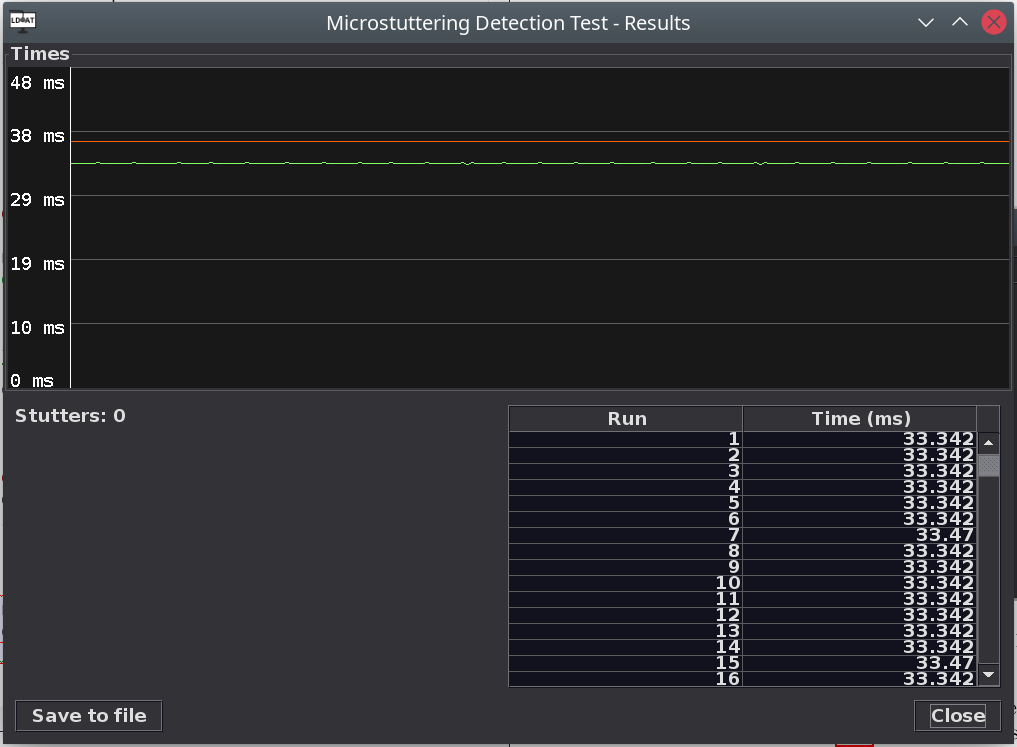
\includegraphics[width=\textwidth]{Applicazione_files/gui_microstuttering_results.png}
	\caption{Rilevamento del microstuttering: risultati del test}
	\label{fig:gui_microstuttering_results}
\end{figure}

\subsubsection{Rilevamento di PWM e noise}
Questo test non ha parametri da configurare, per cui viene eseguito immediatamente. Al termine viene mostrata una schermata con i risultati come in figura \ref{fig:gui_pwm_results}. Da quì è possibile salvarli su un file importabile in un foglio di calcolo oppure tornare al menu principale. Il grafico mostra il segnale catturato dal sensore durante il test.

\begin{figure}[H]
	\centering
	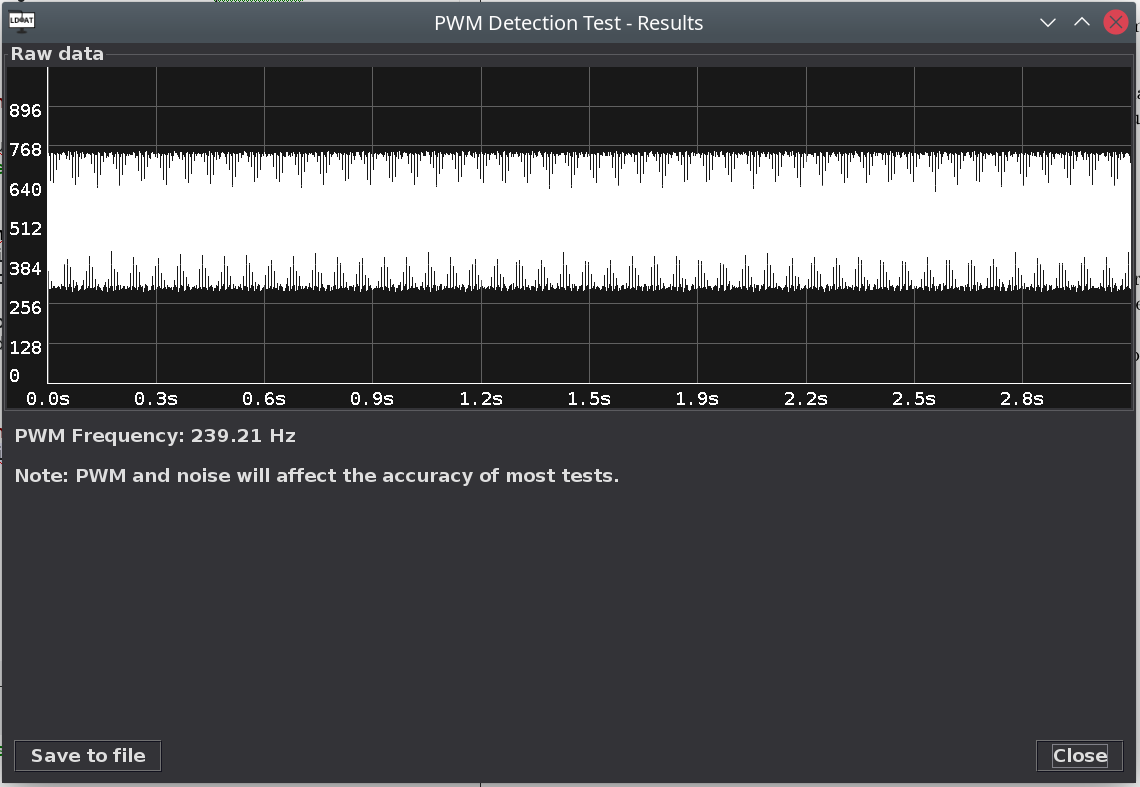
\includegraphics[width=\textwidth]{Applicazione_files/gui_pwm_results.png}
	\caption{Rilevamento di PWM e noise: risultati del test su un display con una pessima retroilluminazione}
	\label{fig:gui_pwm_results}
\end{figure}

\subsubsection{Tempi di risposta dei pixel}
Questo test ha due parametri che possono essere configurati, mostrati in figura \ref{fig:gui_pixelresponse_settings}:\begin{itemize}
	\item \textbf{Evaluation method}: permette di scegliere il range della transizione di cui misurare il tempo. Lo standard VESA prevede di misurare il tempo richiesto per la transizione dal 10\% al 90\%, per cui questo è il default, ma può essere selezionata anche un'altra modalità chiamata umoristicamente ``BS Manufactures Say'' per misurare il range 30\%-70\%, che è più tipicamente usato dai produttori di schermi ``da gaming''
	\item \textbf{Step size}: il passo tra due sfumature di grigio. Valori più piccoli testano più sfumature di grigio ma rendono il test molto più lungo. I valori implementati sono 16 (lento), 32 (default) e 64 (veloce). Questi valori sono su una scala tra 0 e 255 solo per comodità, il test utilizza il formato dei pixel del desktop
\end{itemize}

Al termine del test, viene visualizzata una schermata con i risultati come in figura \ref{fig:gui_pixelresponse_results}. Da quì è possibile salvarli su un file importabile in un foglio di calcolo oppure tornare al menu principale. I colori nella tabella indicano in modo intuitivo quanto è buono il tempo di quella transizione con una sfumatura dal verde al rosso.

Nota: i valori di luminosità sono su una scala tra 0 e 255 solo per comodità, il test utilizza il formato dei pixel del desktop.

\begin{figure}[H]
	\centering
	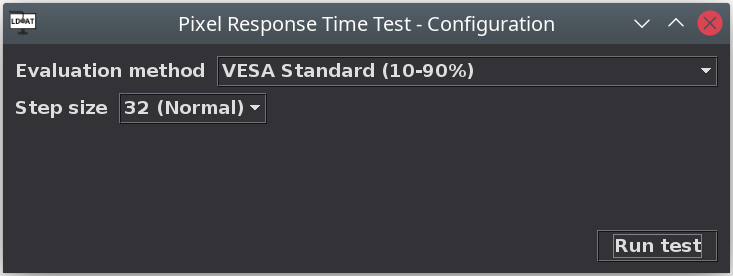
\includegraphics[width=.8\textwidth]{Applicazione_files/gui_pixelresponse_settings.png}
	\caption{Tempi di risposta dei pixel: impostazioni del test}
	\label{fig:gui_pixelresponse_settings}
\end{figure}

\begin{figure}[H]
	\centering
	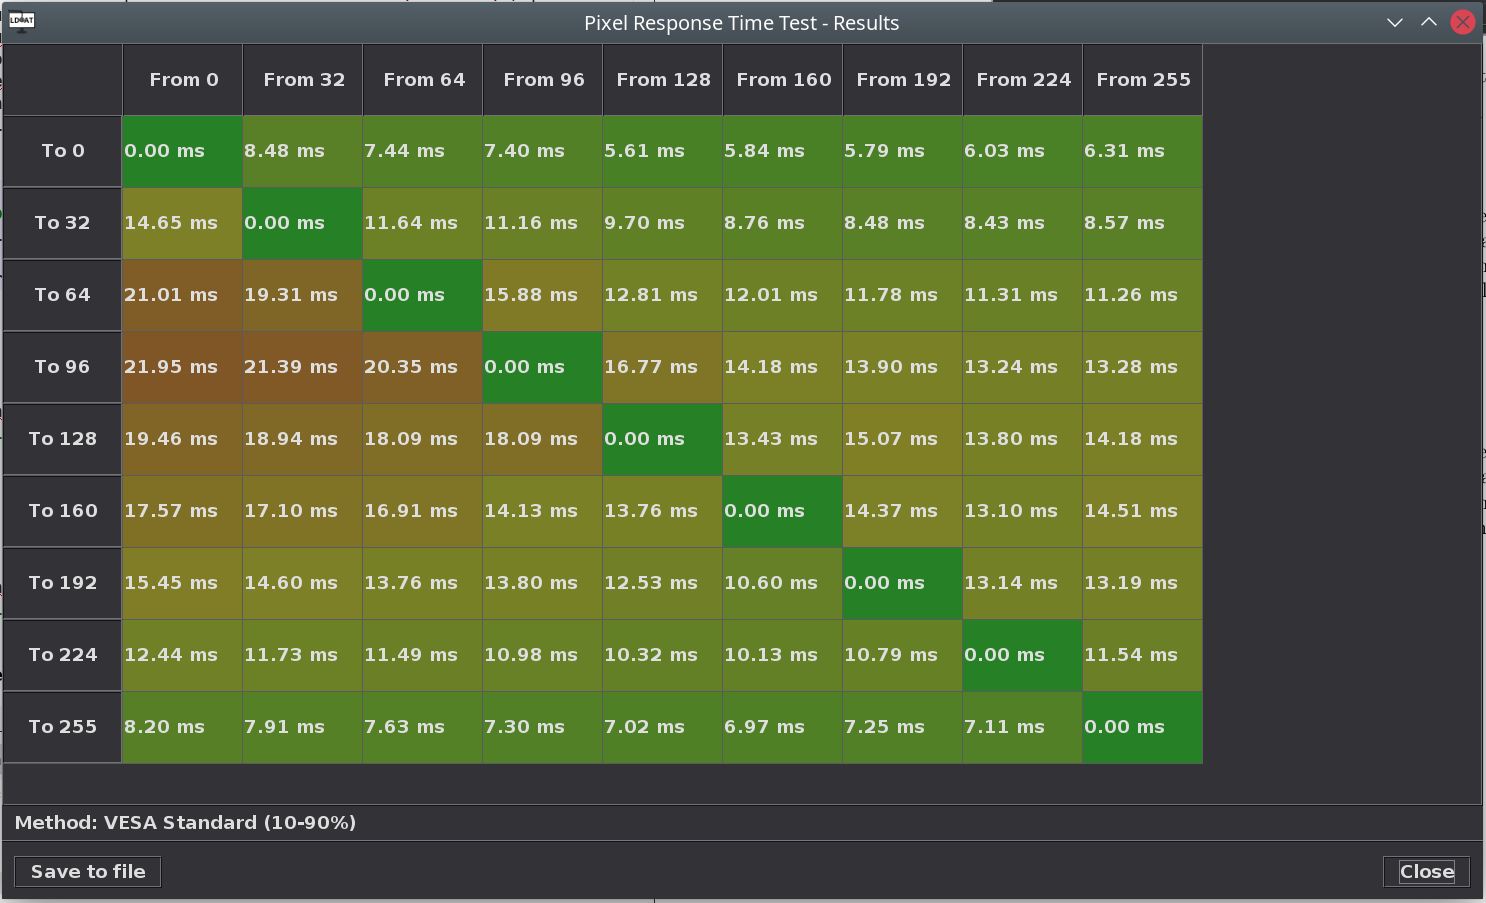
\includegraphics[width=\textwidth]{Applicazione_files/gui_pixelresponse_results.png}
	\caption{Tempi di risposta dei pixel: risultati del test}
	\label{fig:gui_pixelresponse_results}
\end{figure}

\subsubsection{Overdrive dei pixel}
Questo test ha tre parametri che possono essere configurati, mostrati in figura \ref{fig:gui_pixeloverdrive_settings}:\begin{itemize}
	\item \textbf{Method}: permette di scegliere il metodo di misurazione tra Relativo e Assoluto (default), il cui significato è approfondito nella sezione dedicata al funzionamento di questo test
	\item \textbf{Step size}: il passo tra due sfumature di grigio. Valori più piccoli testano più sfumature di grigio ma rendono il test molto più lungo. I valori implementati sono 16 (lento), 32 (default) e 64 (veloce). Questi valori sono su una scala tra 0 e 255 solo per comodità, il test utilizza il formato dei pixel del desktop
	\item \textbf{Skip transitions to 0 and 255}: velocizza il test saltando le transizioni verso il nero e verso il bianco, dato che normalmente il display non può visualizzare colori più scuri del nero o più chiari del bianco
\end{itemize}

Al termine del test, viene visualizzata una schermata con i risultati come in figura \ref{fig:gui_pixeloverdrive_results}. Da quì è possibile salvarli su un file importabile in un foglio di calcolo oppure tornare al menu principale. I colori nella tabella indicano in modo intuitivo quanto è buono il tempo di quella transizione con una sfumatura dal verde al rosso.

Attenzione: questo test è estremamente sensibile alla presenza di PWM o altri disturbi.

Nota: i valori di luminosità sono su una scala tra 0 e 255 solo per comodità, il test utilizza il formato dei pixel del desktop.

\begin{figure}[H]
	\centering
	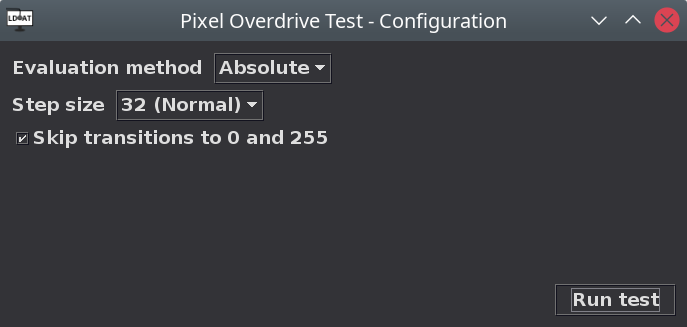
\includegraphics[width=.8\textwidth]{Applicazione_files/gui_pixeloverdrive_settings.png}
	\caption{Overdrive dei pixel: impostazioni del test}
	\label{fig:gui_pixeloverdrive_settings}
\end{figure}

\begin{figure}[H]
	\centering
	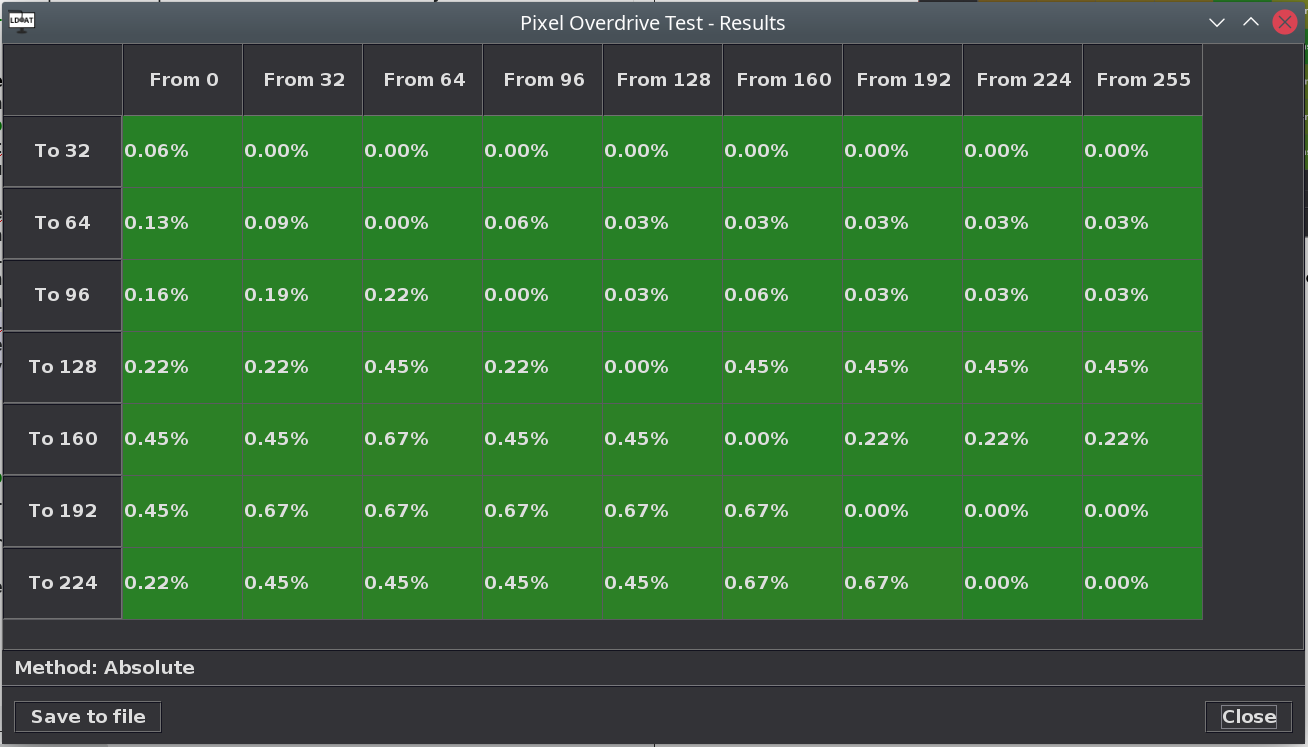
\includegraphics[width=\textwidth]{Applicazione_files/gui_pixeloverdrive_results.png}
	\caption{Overdrive dei pixel: risultati del test}
	\label{fig:gui_pixeloverdrive_results}
\end{figure}

\subsection{Test interattivi}
I test interattivi mostrano una schermata di test in cui è possibile configurarlo mentre il test è in esecuzione. Questi test procedono indefinitamente fino a quando non vengono interrotti dall'utente.

\subsubsection{Input lag (test interattivo)}
Questo test permette di misurare il ritardo in risposta ai click di virtualmente qualsiasi applicazione.

L'interfaccia grafica del test (figura \ref{fig:gui_interactiveinputlag_results}) è organizzata in questo modo:\begin{itemize}
	\item Il grafico mostra i dati del sensore di luminosità (bianco), i click (azzurro), e la soglia di attivazione (linea verde orizzontale)
	\item Alla destra del grafico è possibile regolare la soglia di attivazione con il cursore
	\item Sotto al grafico, sulla destra è possibile cambiare il gain del sensore tra i quattro livelli disponibili e scegliere se i click devono essere generati automaticamente dal dispositivo o se devono essere ricevuti dall'esterno (default)
	\item Sotto al grafico, a sinistra è presente un elenco di tempi misurati finora con la relativa media e la possibilità di salvare i tempi su file e di resettare il test qualora siano stati catturati dati errati
\end{itemize}

\begin{figure}[H]
	\centering
	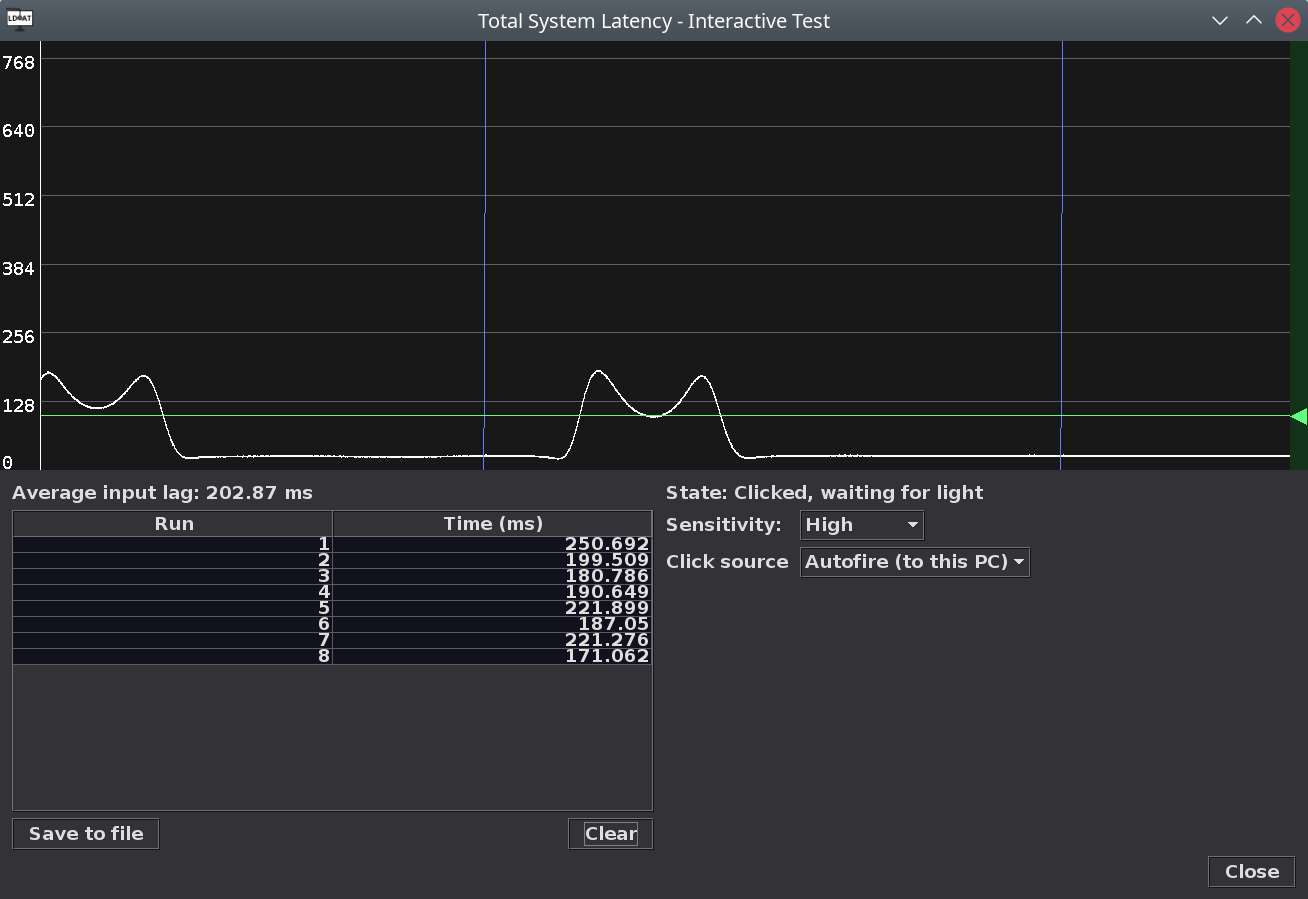
\includegraphics[width=\textwidth]{Applicazione_files/gui_interactiveinputlag_results.png}
	\caption{Input lag (test interattivo): schermata di test}
	\label{fig:gui_interactiveinputlag_results}
\end{figure}

\subsubsection{Light to sound}
Quest'ultimo test permette di ascoltare il segnale del sensore di luminosità come audio.

L'interfaccia grafica del test (figura \ref{fig:gui_lighttosound_results}) è organizzata in questo modo:\begin{itemize}
	\item Il grafico mostra l'ultimo mezzo secondo del segnale catturato
	\item I controlli sotto al grafico permettono di regolare il volume dell'audio e il livello di gain del sensore
	\item Quando viene rilevata una frequenza sufficientemente potente (ad esempio da una retroilluminazione PWM), questa viene mostrata sotto ai controlli
	\item In basso a sinistra viene mostrato il sample rate del segnale catturato
\end{itemize}

\begin{figure}[H]
	\centering
	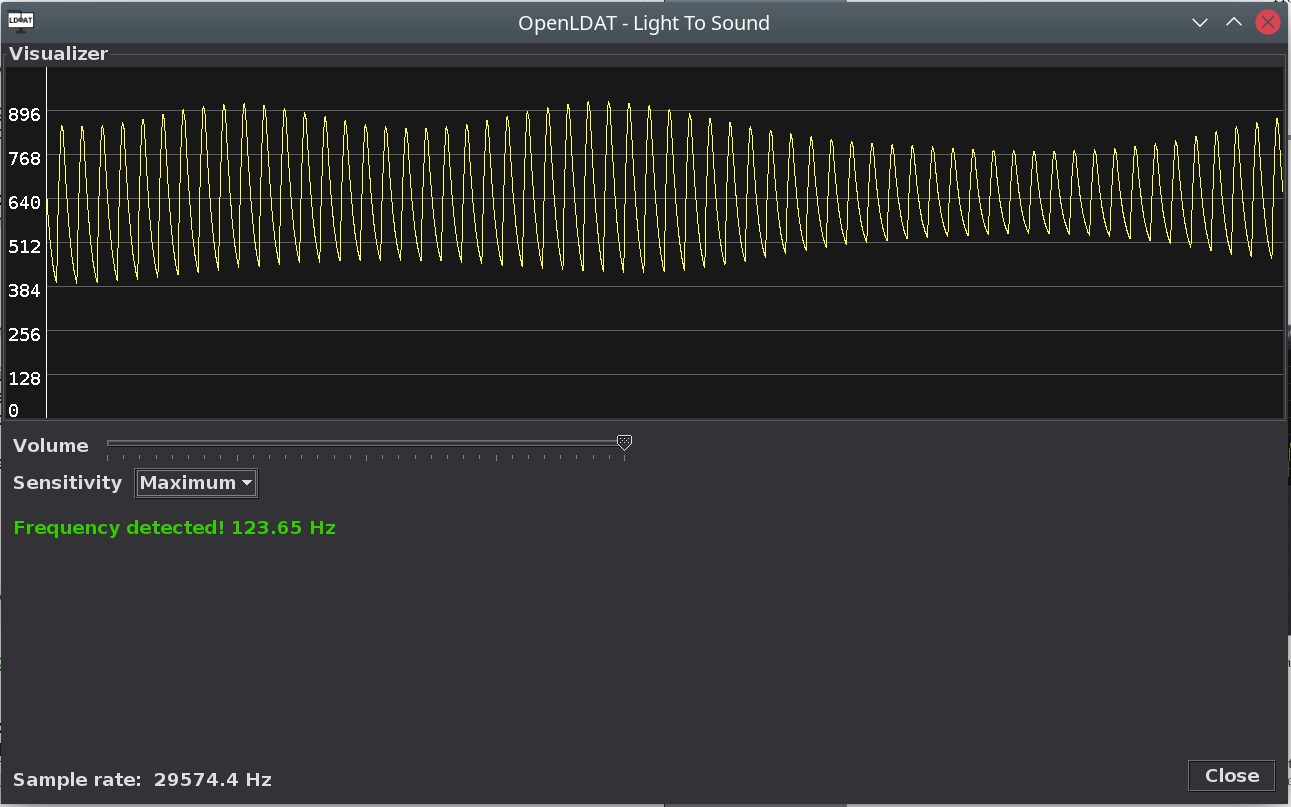
\includegraphics[width=\textwidth]{Applicazione_files/gui_lighttosound_results.png}
	\caption{Light to sound: schermata di test}
	\label{fig:gui_lighttosound_results}
\end{figure}

\subsection{Impostazioni}
La schermata delle impostazioni mostrata in figura \ref{fig:gui_settings} permette di cambiare alcune impostazioni che l'applicazione determina automaticamente:\begin{itemize}
	\item \textbf{Graphics backend}: seleziona il backend grafico tra OpenGL e Swing. Di default viene usato OpenGL se è disponibile, Swing è usato solo come fallback
	\item \textbf{Use antialiasing on charts (slower)}: migliora la qualità dei grafici disegnandoli con l'antialiasing. Di default è disattivato
	\item \textbf{Disable X11 hacks}: permette di disattivare alcuni hack che aumentano la stabilità dell'applicazione su X11 (solo per GNU/Linux). Di default è disattivato
\end{itemize}

Queste impostazioni sono rese disponibili a tutte le classi dell'applicazione sotto forma di variabili statiche nella classe \texttt{Config}, la quale si occupa anche di memorizzarle su disco e applicarle anche ai successivi utilizzi. Le impostazioni sono memorizzate nella cartella \texttt{\textasciitilde/.openldat} (GNU/Linux e MacOS) o \texttt{\%USERPROFILE\%\textbackslash.openldat} (Windows).

\begin{figure}[H]
	\centering
	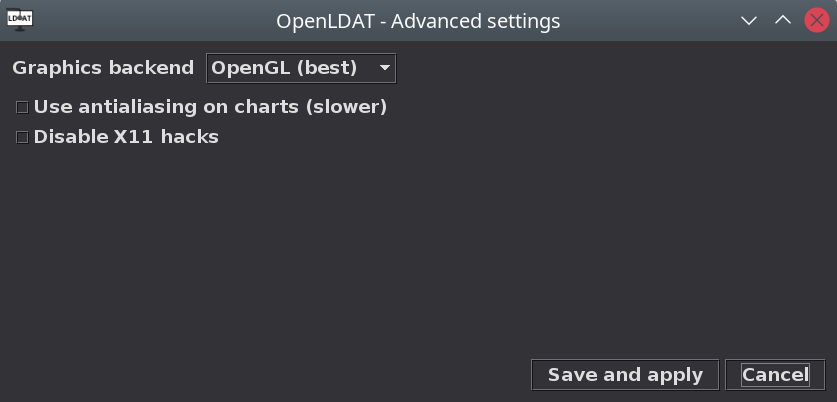
\includegraphics[width=\textwidth]{Applicazione_files/gui_settings.png}
	\caption{Impostazioni dell'applicazione}
	\label{fig:gui_settings}
\end{figure}

\subsection{Schermata about}
Questa schermata mostra le informazioni sull'applicazione: versione, copyright e licenza (GNU GPL Versione 3).

\begin{figure}[H]
	\centering
	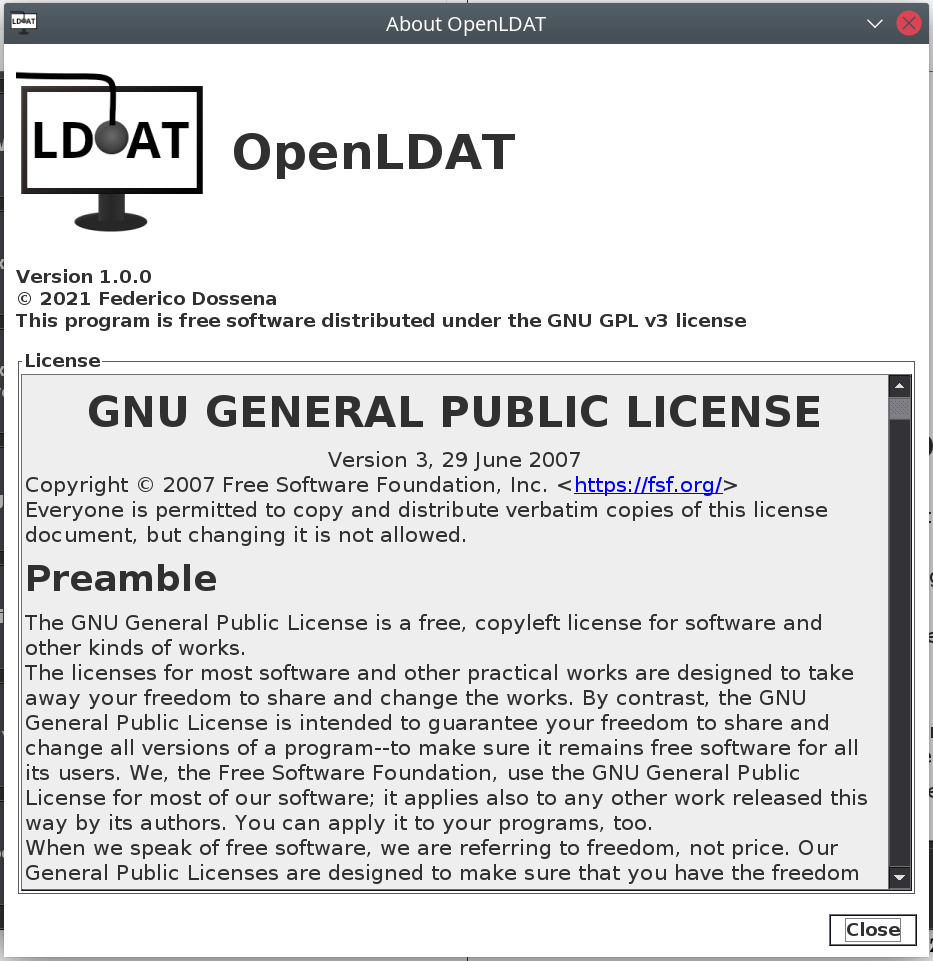
\includegraphics[width=.8\textwidth]{Applicazione_files/gui_about.png}
	\caption{Informazioni su OpenLDAT}
	\label{fig:gui_about}
\end{figure}

Facendo click ripetutamente sul logo di OpenLDAT per 7 volte è possibile accedere al Driver test anche su dispositivi che non sono marcati come prototipi.

\subsection{Gestore grafico degli errori}
L'ultimo componente della GUI è il gestore degli errori. La classe \texttt{ErrorDialog} implementa la schermata di errore in figura \ref{fig:gui_errordialog} e può gestire i seguenti errori:\begin{itemize}
	\item \textbf{Errori dell'applicazione}: file corrotti, applicazione già avviata, crash di thread, eccetera. Questi errori sono critici e causano la chiusura dell'applicazione
	\item \textbf{Errori del dispositivo e del driver}: dispositivi non supportati, disconnessioni inaspettate, risposte non valide del firmware, eccetera. Questi errori sono critici e causano la chiusura dell'applicazione
	\item \textbf{Errori dei test}: fallimenti nell'analisi, contrasto insufficiente, problemi con il backend grafico, sensori mancanti, eccetera. Questi errori causano il fallimento del test, ma l'applicazione può continuare. Alcuni di questi errori, per esempio l'annullamento del test da parte dell'utente, non causano la visualizzazione di un messaggio d'errore
\end{itemize}

\begin{figure}[H]
	\centering
	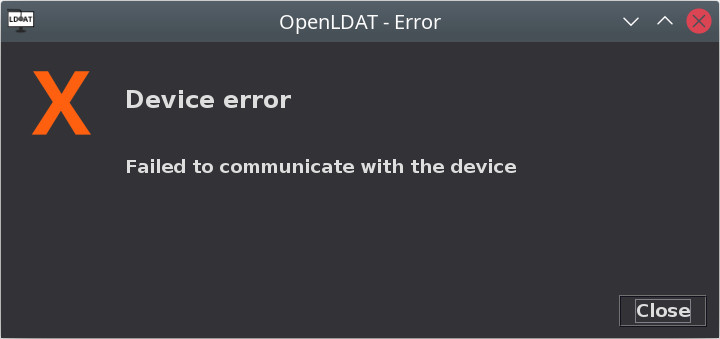
\includegraphics[width=.8\textwidth]{Applicazione_files/gui_errordialog.png}
	\caption{Schermata di errore di OpenLDAT}
	\label{fig:gui_errordialog}
\end{figure}

Un errore che viene trattato in modo speciale da questa classe è quello che si verifica se il dispositivo viene rilevato ma l'utente corrente non ha i permessi per comunicare con esso. Questo è un problema che si verifica su alcune distribuzioni di GNU/Linux e l'applicazione implementa una schermata di errore speciale (figura \ref{fig:gui_linuxerror}) che si offre di correggere i permessi automaticamente tramite uno script (se l'utente è amministratore) o di mostrare istruzioni su come farlo manualmente da un terminale.\\
Lo script automatico supporta distribuzioni GNU/Linux basate su Debian, Arch, SUSE e RedHat, ed è stato testato su Ubuntu 21.04, Debian 10.9, Manjaro 21, Arch Linux (Aprile 2021), OpenSUSE 15, Fedora 34.

\begin{figure}[H]
	\centering
	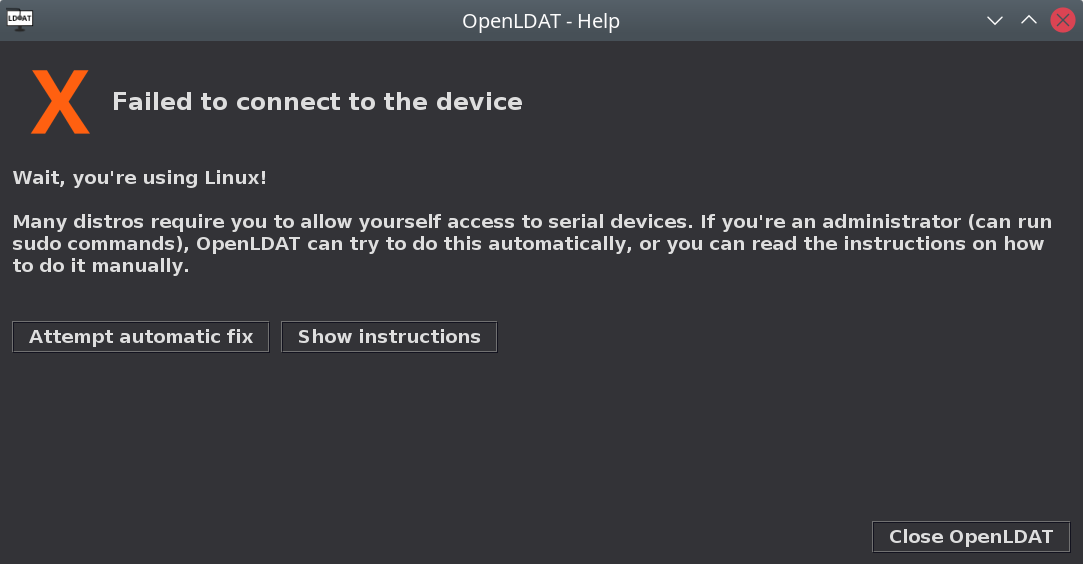
\includegraphics[width=\textwidth]{Applicazione_files/gui_linuxerror.png}
	\caption{Correzione automatica dei permessi mancanti su GNU/Linux}
	\label{fig:gui_linuxerror}
\end{figure}

Questo conclude la sezione di presentazione dell'interfaccia grafica dell'applicazione OpenLDAT.

\section{Packaging dell'applicazione}
Per consentire un facile utilizo dell'applicazione, soprattutto da utenti inesperti, è necessario creare dei pacchetti binari per le varie piattaforme. Sono stati scelti i seguenti target:\begin{itemize}
	\item Windows 10 x64
	\item GNU/Linux amd64 (diverse distribuzioni popolari)
	\item MacOS Intel 64 bit
\end{itemize}
Essendo il codice multipiattaforma, è possibile utilizzarlo anche su altre piattaforme come BSD o Windows a 32 bit, tuttavia queste non sono state testate e non si garantisce il corretto funzionamento.

Tutti i file e le istruzioni necessarie per il packaging sulle piattaforme target sono presenti nella cartella \texttt{Packaging stuff} all'interno della cartella dell'applicazione.

\subsection{Windows}
Il pacchetto di installazione per Windows è stato realizzato utilizzando Inno Setup\footnote{\href{https://jrsoftware.org/isinfo.php}{https://jrsoftware.org/isinfo.php}}. All'interno del package sono presenti l'applicazione OpenLDAT con le relative librerie, il runtime Java (OpenJDK 11 JRE\footnote{\href{https://adoptopenjdk.net/releases.html}{https://adoptopenjdk.net/releases.html}}), e un launcher eseguibile per Windows realizzato con Launch4J\footnote{\href{https://launch4j.sourceforge.net/}{https://launch4j.sourceforge.net/}}.

La procedura per realizzare il package è la seguente:\begin{itemize}
	\item Fare una copia della cartella \texttt{Windows-InnoSetup}
	\item Eseguire la build del progetto OpenLDAT da NetBeans IDE
	\item Dalla cartella \texttt{dist} nel progetto appena compilato, copiare \texttt{OpenLDAT.jar} e la cartella \texttt{lib} nella cartella \texttt{openldat}
	\item Scaricare il file zip di OpenJDK JRE x64 versione 11 o superiore dal relativo sito
	\item All'interno dello zip scaricato estrarre i file del runtime (cartelle \texttt{bin}, \texttt{lib}, eccetera) nella cartella \texttt{jre}
	\item Utilizzando Launch4J, eseguire la build del file \texttt{launcher.xml}
	\item Utilizzando Inno Setup 6, eseguire la build del file \texttt{setup.iss}. Al termine verrà generato un file chiamato \texttt{OpenLDAT\_Setup.exe} che può essere distribuito. Si consiglia di firmarlo digitalmente
\end{itemize}

\subsection{GNU/Linux}
Il pacchetto per GNU/Linux è distribuito nel formato AppImage\footnote{\href{https://appimage.org/}{https://appimage.org/}}, che non richiede installazione. All'interno del package sono presenti l'applicazione OpenLDAT con le relative librerie e il runtime Java (OpenJDK 11 JRE).

La procedura per realizzare il package è la seguente:\begin{itemize}
	\item Fare una copia della cartella \texttt{Linux-AppImage} ed entrare nella cartella \texttt{OpenLDAT.AppDir}
	\item Eseguire la build del progetto OpenLDAT da NetBeans IDE
	\item Dalla cartella \texttt{dist} nel progetto appena compilato, copiare \texttt{OpenLDAT.jar} e la cartella \texttt{lib} nella cartella \texttt{openldat}
	\item Scaricare il file zip di OpenJDK JRE x64 versione 11 o superiore dal relativo sito
	\item All'interno dello zip scaricato estrarre i file del runtime (cartelle \texttt{bin}, \texttt{lib}, eccetera) nella cartella \texttt{jre}
	\item Tornare al livello superiore ed eseguire il seguente comando:\begin{verbatim}
		appimagetool OpenLDAT.AppDir
	\end{verbatim}
	Al termine verrà generato un file chiamato \texttt{OpenLDAT-x86\_64.AppImage} che può essere distribuito
\end{itemize}

\subsection{MacOS}
Il pacchetto per MacOS è distribuito sotto forma di immagine DMG contenente un'applicazione nel formato standard .app, la quale contiene al suo interno l'applicazione OpenLDAT con le relative librerie, il runtime Java (OpenJDK 11 JRE), e un wrapper per consentire l'avvio di applicazioni Java su MacOS\footnote{\href{https://github.com/tofi86/universalJavaApplicationStub}{https://github.com/tofi86/universalJavaApplicationStub}}.

Nota: il testing su questa piattaforma è stato estremamente limitato e non è stato eseguito dall'autore di questa tesi.

La procedura per realizzare il package è la seguente:\begin{itemize}
	\item Fare una copia della cartella \texttt{Mac}
	\item Eseguire la build del progetto OpenLDAT da NetBeans IDE
	\item Dalla cartella \texttt{dist} nel progetto appena compilato, copiare \texttt{OpenLDAT.jar} e la cartella \texttt{lib} nella cartella \texttt{openldat}
	\item Scaricare il file zip di OpenJDK JRE x64 versione 11 dal relativo sito\\
	Attenzione: La versione 11 è l'unica supportata da questo sistema di packaging al momento
	\item All'interno dello zip scaricato estrarre i file del runtime (cartelle \texttt{bin}, \texttt{lib}, eccetera) nella cartella \texttt{jre/openjdk-11-jre}
	\item Eseguire lo script \texttt{makeapp}. Al termine verrà generata una cartella \texttt{OpenLDAT.app}
	\item Utilizzare Disk Utility per creare un'immagine DMG compressa contenente \texttt{OpenLDAT.app} che può essere distribuita
\end{itemize}

Questo conclude il capitolo sull'applicazione OpenLDAT per PC. Nel capitolo successivo verranno mostrati e discussi alcuni risultati raccolti con l'applicazione e il dispositivo in diversi scenari.
